% INHALT: {{{
% Material und Methoden:
% - technische Ausrüstung, Rechen-, Messmethoden, Auswerteverfahren etc., die in der Arbeit verwendet wurden
% Ergebnisse bzw. Resultate:
% - Beschreibung bzw. Darstellung der erzielten Ergebnisse
% }}}

\subsection{Material und Methoden}

\subsubsection{Technische Ausrüstung \& Verwendete Tools} %{{{

Alles was verwendet wurde ist in \tabref{table:Tools} aufgelistet.

\begin{center}
    \begin{tabular}{ | >{\RaggedRight\hspace{0pt}} l|l | }
        \hline
        \textbf{Programme} & \\
        KiCAD \cite{kicad}                  & Schema- \& Leiterplatten-Designer \\
        STM32CubeIDE \cite{stm32cube}       & Programmierumgebung von ST \\
        Fusion 360 \cite{fusion}            & 3D-Konstruktions-Software \\
        Prusa Slicer \cite{prusa-slicer}    & Preparation von Objekten zum 3D-Druck \\
        LibreOffice \cite{libreoffice}      & Präsentationen (Exposé) \\
        MobaXTerm \cite{mobaxterm}          & Kommunikation über serielle Schnittstellen \\
        Excalidraw \cite{excalidraw}        & Diagramme \\
        Python \cite{python}                & Programmiersprache \\
        C/C++ \cite{cpp}                    & Programmiersprache \\
        \hline
        \textbf{Programmier-Bibliotheken}   & \\
        opencv \cite{opencv}                & Bildverarbeitungs-Bibliothek \\
        numpy \cite{numpy}                  & Numerische Rechenbibliothek \\
        matplotlib \cite{mpl}               & Bibliothek zum grafischen darstellen von Daten \\
        scipy \cite{scipy}                  & Algorithmen für Wissenschaftliches Rechnen \\
        \hline
        \textbf{Allgemeines} & \\
        vim \cite{vim}, neovim \cite{neovim}        & Text- \& Code-Editor \\
        git \cite{git}, GitHub \cite{github}        & Versionierungs-Software \& Datenbank \\
        Linux \cite{linux}, Windows \cite{windows}  & Betriebssystem \\
        \hline
        \textbf{Hardware} & \\
        Keysight MSOX3024T \cite{voltcraft} & Oszilloskop \\
        \hypertarget{hyp:Prusa-MK4}{Prusa MK4} \cite{prusa-mk4} & 3D-Drucker \\
        \hypertarget{hyp:IDS}{IDS} UI-3250CP-M-GL \cite{ids} & Kamera \\
        \hypertarget{hyp:AOS}{AOS} U750 COLOR \cite{aos} & Kamera \\
        Samsung Galaxy \hypertarget{hyp:A52}{A52} \cite{a52} & Kamera \\
        \hline
    \end{tabular}
    \captionof{table}{Technische Ausrüstung \& Verwendete Tools}
    \label{table:Tools}
\end{center}

\subsubsection{Entwicklungsprozess der Hardware}

Die Hardware wurde iterativ entwickelt.
Zu Beginn wurde das Schieberegister auf einem Steckbrett ausgetestet.
Danach konnte ein Schema und Layout im KiCad gezeichnet werden, welches dann von JLCPCB \cite{jlc} hergestellt wurde.
Bauteile wurden entweder von der Schule bezogen oder von DigiKey \cite{digikey} bestellt.
In der ersten PCB (Printed Circuit Board) Version war noch kein Kommunikationsport vorhanden, es hatte noch keinen externen Oszillator und noch diverse Speisungsfehler für den Mikrokontroller.
In der zweiten Version wurde dies behoben. Dennoch hat es noch einen kleinen Fehler, der Ausgebessert werden musste, damit die USB-Kommunikation einwandfrei funktioniert.
Die im \appref{app:hw-ledrunner} beigelegte Version enthält alle Verbesserungen.

\subsubsection{Entwicklungsprozess der Software}

Die Software wurde ebenfalls iterativ entwickelt \cite{stackoverflow,stackexchange,mathexchange,geeks}.
Zuerst entstand die Auswertung für eine LED-Helligkeitskalibration (\appref{app:camera-calibration}), der \secref{sec:Machbarkeitsanalyse-der-Kalibration} geht näher darauf ein.
Danach entstand eine Version, in der noch keine Kalibration durchgeführt wurde und die Position des Gerätes von Hand eingezeichnet werden musste (\appref{app:eval-static}).
Darin befindet sich der erste Ansatz zur Auswertung eines Messvideos.
In der aktuellen Version der Auswertungssoftware (\appref{app:eval-dynamic}) wurden die beiden Teile zusammengeführt.
Damit erfolgt die Auswertung nun vollautomatisch, denn das Messgerät wird gefunden, und ebenso eine Helligkeitskalibration durchgeführt.

Für den ersten Teil ist die Mikrokontroller-Software im \appref{app:sw-camera-calibration} erstellt worden.
Danach wurde eine separate Version kontinuierlich erweitert in \appref{app:sw-ledrunner}.
Dies ist gleichzeitig die aktuelle Version.



\subsubsection{Entwicklungsprozess des Gehäuses}

Das Gehäuse wurde, wie auch die Hardware und Software, iterativ entwickelt.
Die ersten paar Versionen hatten zu kleine Toleranzen und es schlichen sich Logikfehler ein.
Die aktuelle Version im \appref{app:housing-ledrunner} passte schlussendlich.
Der \hyperlinkXY{hyp:Prusa-MK4} wurde verwendet um dies physikalisch zu erstellen.

% END: Verwendete Tools }}}

\subsection{Kalibrationsgerät} %{{{

Ein Kalibrationsgerät wurde entwickelt, welches die Auswerteverfahren in \secref{sec:Auswerteverfahren} ermöglicht.

\subsubsection{Blockschaltbild}

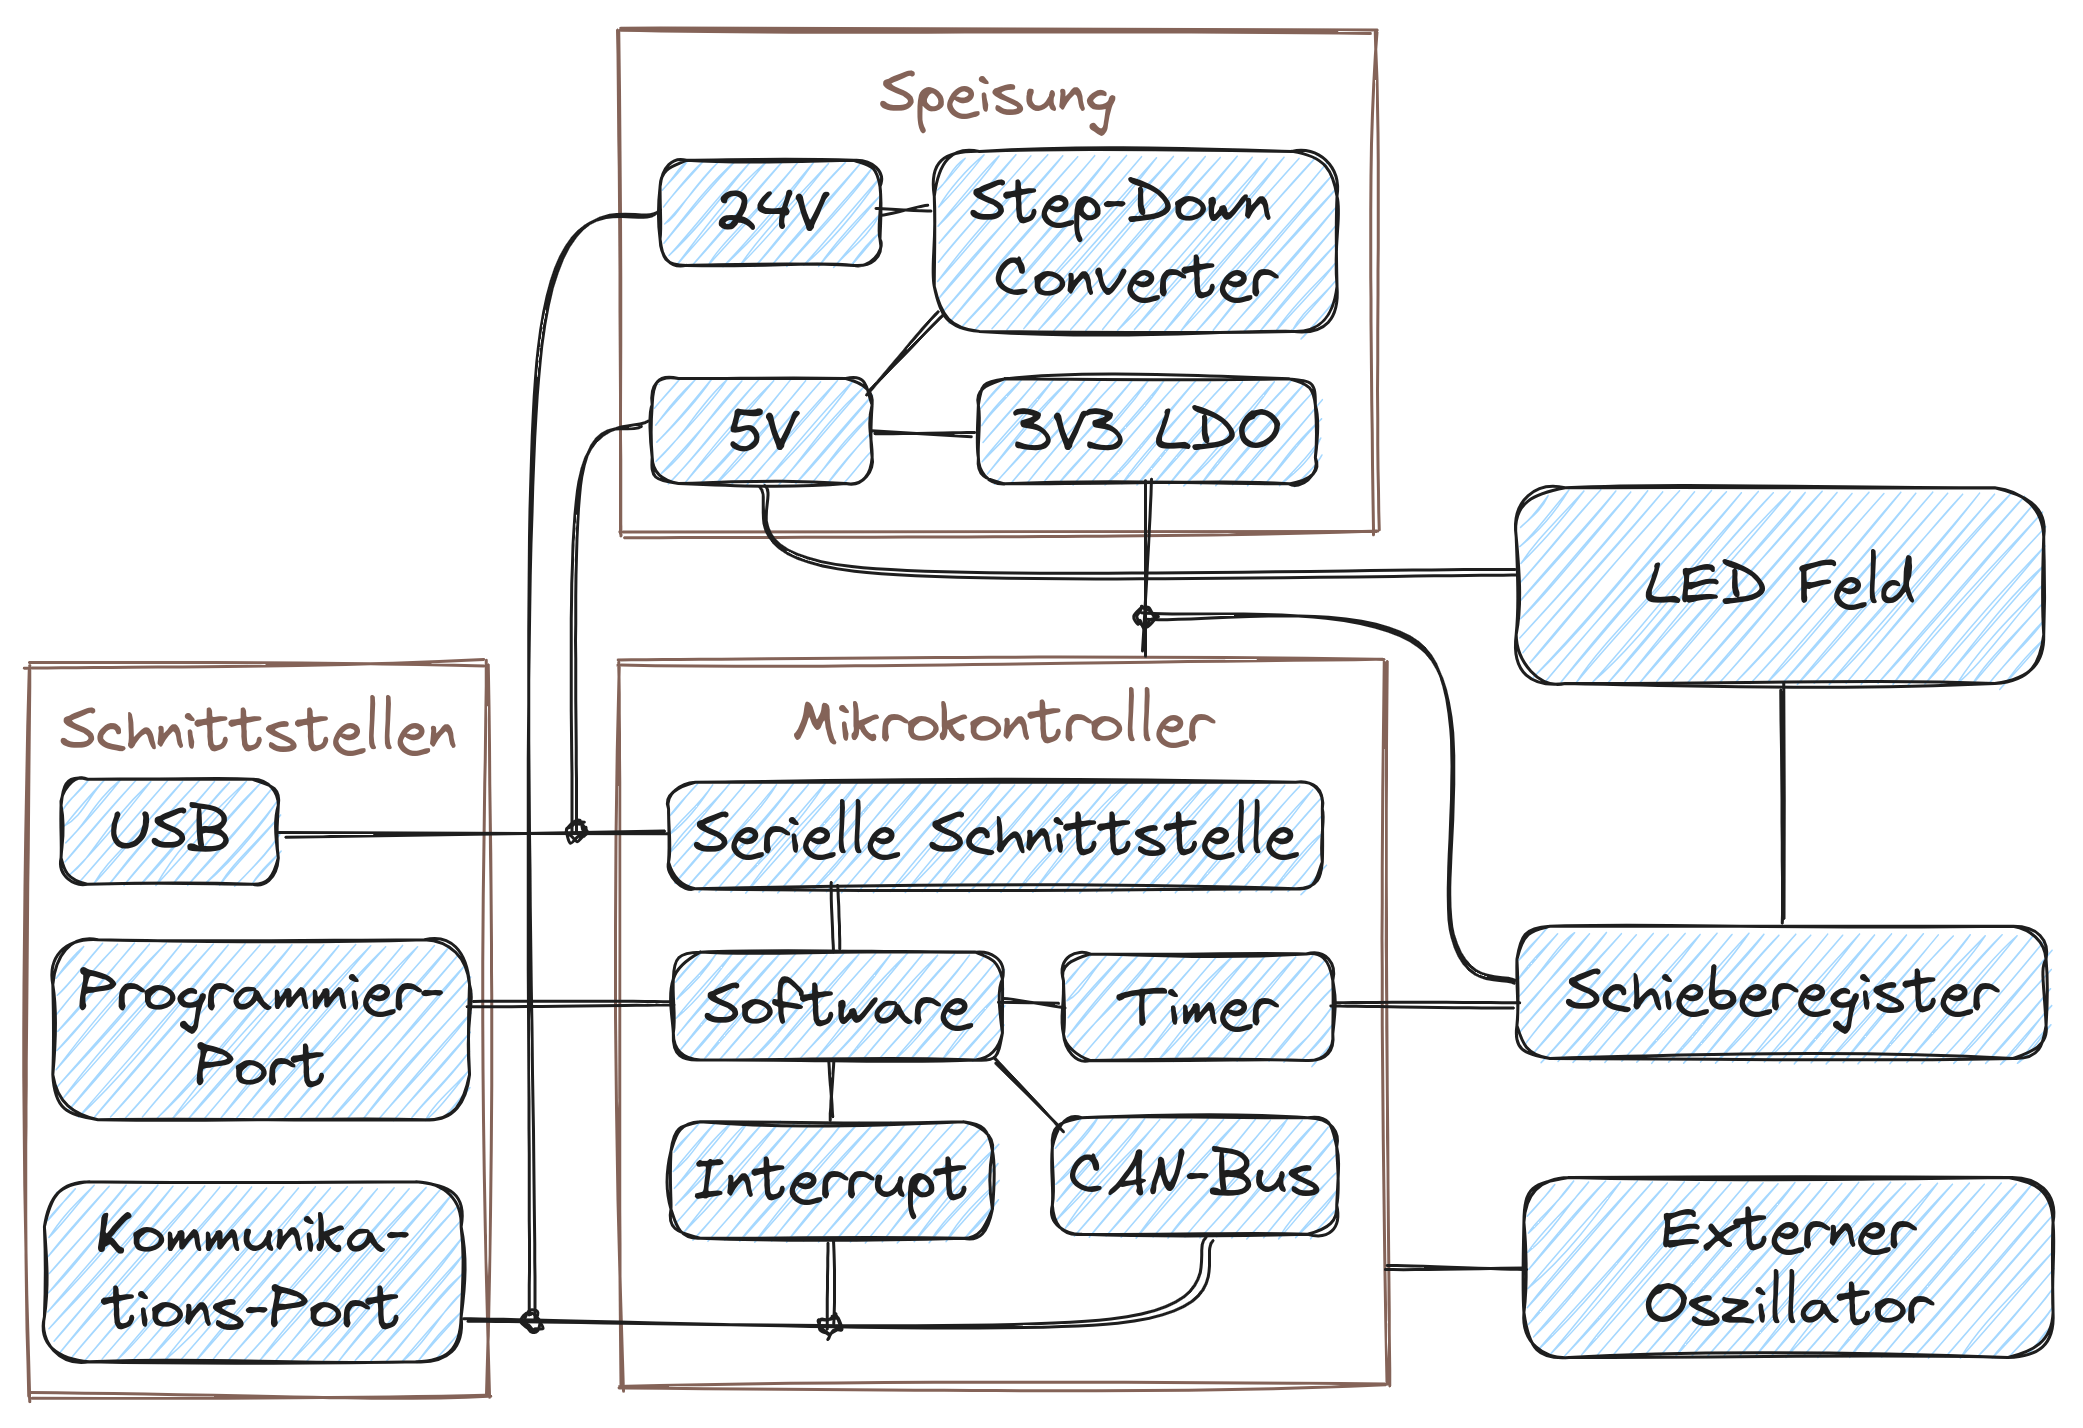
\includegraphics[width=\linewidth]{../images/blockschaltbild.png}
\vspace{-3em}
\captionof{figure}{Blockschaltbild}
\vspace{0.5em}
\label{img:Blockschaltbild}

Diverse Punkte von \imgref{img:Blockschaltbild} genauer betrachtet:
%\tablevspaceASenum
\begin{longtable}[l]{ @{} >{\RaggedRight\hspace{0pt}} lp{.96\linewidth} @{} }
    \textbullet & Für den Mikrokontroller ist ein STM32 mit einer Taktgeschwindigkeit von 72MHz vorgesehen.
    \\\textbullet & Das Schieberegister fungiert auch direkt als Stromtreiber für die LEDs. Die maximale Taktgeschwindigkeit dessen beträgt 30MHz.
    \\\textbullet & Kommunikation mit dem PC geschieht über den USB-Port per serieller Schnittstelle.
    \\\textbullet & Kommunikation mit anderen Kalibrationsgeräten geschieht über den Kommunikations-Port per CAN-Bus \textit{(noch nicht implementiert)}. Ein Interrupt soll auf eine konfigurierbare Aktion belegt werden können, zum Beispiel als externer Trigger \textit{(aktuell nur belegbar auf den \hyperlinkXY{hyp:mode-auto} Modus)}.
    \\\textbullet & Es ist möglich das Gerät über USB oder eine 24V-Speisung zu betreiben.
    \\\textbullet & Um eine möglichst genaue Taktrate zu erzielen wird ein externer Oszillator verwendet.
    \addtocounter{table}{-1}\setcounter{enumi}{0}
\end{longtable}
\tablevspaceASenum

\subsubsection{Hard- \& Software}

Alles bezüglich der Hardware (Schema und Layout) ist im \appref{app:hw-ledrunner}.
Das PCB ist in \imgref{img:PCB} gezeigt und beschrieben.
Das Gehäuse ist im \appref{app:housing-ledrunner}.
Die gesamte Software des Messgeräts ist im \appref{app:sw-ledrunner}.

\vspace{1em}
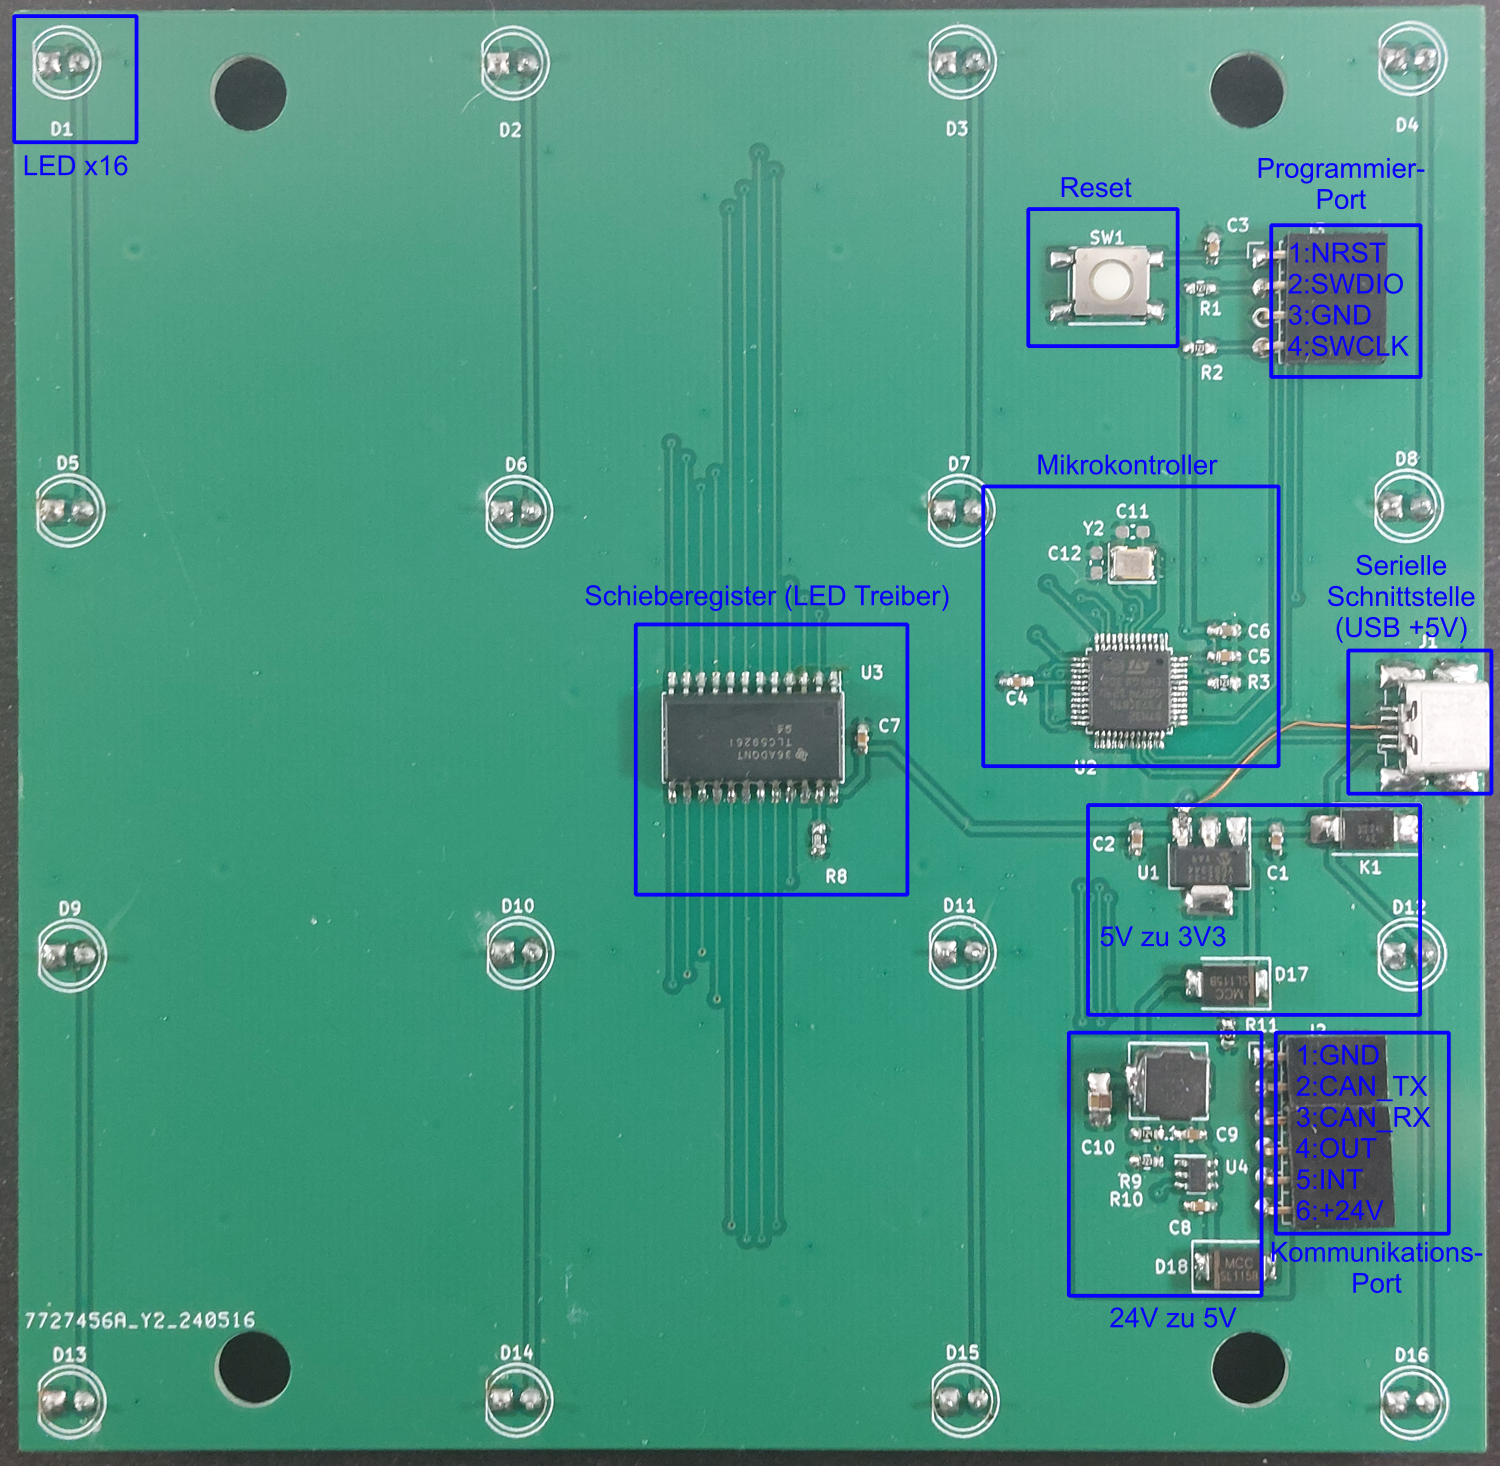
\includegraphics[width=\linewidth]{../images/phone/pcb-edit.png}
\vspace{-2.5em}
\captionof{figure}{PCB}
\label{img:PCB}

\subsubsection{Anordnung der Leuchtdioden}

Verschiedene grössen von quatratischen Anordnungen wurden in Betracht gezogen.
%
Der grösste Einfliessende Faktor ist jedoch die Anzahl an Ausgängen vom Schieberegister.
%
Das ausgesuchte Schieberegister besitzt 16 Ausgänge.
%
Somit kann passend ein Feld bestehend aus 4x4, also insgesamt 16 LEDs, aufgebaut werden.


\subsubsection{Kodierung der Zeit}

Die erste Idee war, dass ein Zeitstempel, ähnlich wie bei QR-Codes (quick-response code) oder Data-Matrizen, angezeigt wird.
%
Dies müsste dann mit der Frequenz abgestimmt werden und es hätte in jedem Bild einen unverwechselbaren Zeitstempel.
%
Kompliziert wird es jedoch, wenn die Kamera durch die Belichtungszeit mehrere Zeitstempel ineinenader verwischen lässt.


Der zweite und ausgewählte Ansatz ist das ``wandern'' lassen einer LED.
%
Es soll also zu jedem Zeitpunkt immer nur eine LED leuchten.
%
Die Geschwindigkeit der ``Wanderung'' wird abgestimmt auf die Aufnahmefrequenz, so dass einmal das gesamte Feld innerhalb von einer zur nächsten Bildaufnahme besucht wird (siehe \secref{sec:Gut-Eingestellt}).
%
Damit lässt sich in der Video-Analyse anhand von Änderungen in der Position der LEDs die Stabilität ausfindig machen.
%
Durch die Anzahl an leuchtenden LEDs im Messvideo lässt sich die Belichtungszeit ermitteln.

\subsubsection{Infobefehle}

Über die serielle Schnittstelle sind die Infobefehle aus \tabref{table:Liste-der-Infobefehle} zur Verfügung gestellt.

\tablevspaceAStable
\begin{tabular}{ @{} >{\RaggedRight\hspace{0pt}} ll @{} }
    Befehl & Zweck \\
    \hline
    \texttt{info} & Auflistung aller Infobefehle \textit{(dies ist als Hilfestellung gegeben)} \\
    \texttt{info version} & Ausgabe der aktuellen Version \\
    \texttt{info arr} & Ausgabe der \hyperlinkXY{hyp:config-arr} Konfiguration \\
    \texttt{info psc} & Ausgabe der \hyperlinkXY{hyp:config-psc} Konfiguration \\
    \texttt{info fps} & Ausgabe der \hyperlinkXY{hyp:config-fps} Konfiguration \\
    \texttt{info out} & Ausgabe der \hyperlinkXY{hyp:config-out} Konfiguration \\
    \texttt{info int} & Ausgabe der \hyperlinkXY{hyp:config-int} Konfiguration \\
    \texttt{info all} & Informationen von allem anzeigen \\
\end{tabular}
\captionof{table}{Liste der Infobefehle}
\label{table:Liste-der-Infobefehle}

\subsubsection{Konfigurationsmöglichkeiten}

Über die serielle Schnittstelle sind die Konfigurationsbefehle aus \tabref{table:Ansteuerung-der-Konfiguration} zur Verfügung gestellt.

\tablevspaceAStable
\begin{tabular}{ @{} >{\RaggedRight\hspace{0pt}} ll @{} }
    Befehl & Zweck \\
    \hline
    \texttt{config} & Auflistung der Konfigurationsbefehle \textit{(dies ist als Hilfestellung gegeben)} \\
    \texttt{config }\hypertarget{hyp:config-fps}{\texttt{fps}}\texttt{=ZAHL} & Setzen der Schaltfrequenz einer einzelnen LED im \hyperlinkXY{hyp:mode-rider} Modus \\
    \texttt{config }\hypertarget{hyp:config-arr}{\texttt{arr}}\texttt{=ZAHL} & Manuelles einstellen vom Auto-Reload des Timers \\
    \texttt{config }\hypertarget{hyp:config-psc}{\texttt{psc}}\texttt{=ZAHL} & Manuelles einstellen vom Prescaler des Timers \\
    \texttt{config }\hypertarget{hyp:config-int}{\texttt{int}}\texttt{=on/off} & Ein- oder ausschalten des GPIO Interrupts zum Start vom \hyperlinkXY{hyp:mode-auto} Modus \\
    \texttt{config }\hypertarget{hyp:config-out}{\texttt{out}}\texttt{=on/off} & Ein- oder ausschalten des GPIO Ausgangs beim Start vom \hyperlinkXY{hyp:mode-auto} Modus \\
    \texttt{config }\hypertarget{hyp:config-reset}{\texttt{reset}} & Reset auslösen \\
\end{tabular}
\captionof{table}{Ansteuerung der Konfiguration}
\label{table:Ansteuerung-der-Konfiguration}

\tablevspaceASenum
\begin{longtable}[l]{ @{} >{\RaggedRight\hspace{0pt}} lp{.96\linewidth} @{} }
    \textbullet & Die \hyperlinkXY{hyp:config-fps} Konfiguration versucht möglichst nahe an die gewünschte FPS (Bilder pro Sekunde) heranzukommen und setzt den Auto-Reload und Prescaler automatisch.
    \\\textbullet & Wird \hyperlinkXY{hyp:config-arr} oder \hyperlinkXY{hyp:config-psc} verändert, aktualisiert dies die \hyperlinkXY{hyp:config-fps} gemäss \eqref{eq:f_Timer}.
  \addtocounter{table}{-1}\\
\end{longtable}
\tablevspaceASenum


\subsubsection{Modi}\label{sec:Modi}

Das Gerät kann in verschiedene Modi gesetzt werden, die alle einen bestimmten Zweck erfüllen, welche in \tabref{table:Ansteuerung-der-Modi} aufgelistet sind.

\tablevspaceAStable
\begin{tabular}{ @{} >{\RaggedRight\hspace{0pt}} ll @{} }
    Befehl & Zweck \\
    \hline
    \texttt{mode} & Auflistung der Modi \textit{(dies ist als Hilfestellung gegeben)} \\
    \texttt{mode }\hypertarget{hyp:mode-none}{\texttt{none}} & Alle LEDs aus \\
    \texttt{mode }\hypertarget{hyp:mode-pwm}{\texttt{pwm}}\texttt{=ZAHL} & Alle LEDs über PWM ansteuern \\
    \texttt{mode }\hypertarget{hyp:mode-display}{\texttt{display}}\texttt{=BINÄRZAHL} & Eine Zahl anzeigen \\
    \texttt{mode }\hypertarget{hyp:mode-rider}{\texttt{rider}} & Eine LED wandern lassen \\
    \texttt{mode }\hypertarget{hyp:mode-auto}{\texttt{auto}} & Automatisches abspielen der Modi (siehe \secref{sec:Reihenfolge-der-Modi}) \\
\end{tabular}
\captionof{table}{Ansteuerung der Modi}
\label{table:Ansteuerung-der-Modi}

\tablevspaceASenum
\begin{longtable}[l]{ @{} >{\RaggedRight\hspace{0pt}} lp{.96\linewidth} @{} }
    \textbullet & Im \hyperlinkXY{hyp:mode-pwm} Modus kann eine Zahl zwischen 0 bis und mit 16 angegeben werden. Somit gibt dies 17 Stufen (siehe \secref{sec:PWM-Modus}). \\
    \textbullet & Im \hyperlinkXY{hyp:mode-display} Modus muss mindestens eine 16-stellige Binärzahl angegeben werden, bei der jedes Bit einer LED entspricht. Alles nach 16 Bits wird ignoriert. Beispiel: \texttt{mode display=1010010111110000}.
    \addtocounter{table}{-1}\\
\end{longtable}
\tablevspaceASenum

%}}}

\subsection{Rechenmethoden} %{{{

Aus den aktiven Leuchtdioden können zwei grundlegende Informationen extrahiert werden:

\tablevspaceASenum
\begin{tabular}{ @{} >{\RaggedRight\hspace{0pt}} lll @{} }
    \refstepcounter{enumi}\theenumi. & Bildwiederholrate & Zentrum der aktiven Leuchtdioden, siehe \secref{sec:Zentrum-def-laufenden-Leuchtdiode}
    \\\refstepcounter{enumi}\theenumi. & Belichtungszeit & Breite der aktiven Leuchtdioden, siehe \secref{sec:Breite-der-laufenden-Leuchtdiode}
\end{tabular}
\tablevspaceASenum

Da die Auswertung über mehrere Bilder geschieht, kann über die Stabilität der Bildwiederholrate und der Belichtungszeit beurteilt werden \textit{(Jitter)}.

%}}}

\subsection{Messmethoden} %{{{

\subsubsection{Machbarkeitsanalyse der Kalibration}\label{sec:Machbarkeitsanalyse-der-Kalibration}

    Zu Beginn war unbekannt, ob es Sinn machen würde, die Helligkeiten der LEDs zu kalibrieren, und ob dies überhaupt funktioniert.
    Deshalb wurden auf einer LED eines STM32 Nucleo Boards verschiedene Helligkeitsstufen mittels PWM eingestellt. Eine Kamera nahm Bilder davon auf und die Helligkeiten wurden ausgewertet.

    In \imgref{img:PWM-Machbarkeitsanalyse} sind die Verläufe, nebst einer Ideallinie, eingezeichnet.
    Es ist ersichtlich, dass eine Helligkeits, bzw. PWM-Kalibration potentiellen nichtlinearitäten entgegenwirken könnte.
    Es kommt ebenso darauf an, wie gross die auszuwertende Fläche in Pixel ist, welche in \imgref{img:PWM-Machbarkeitsanalyse-Flächen} dargestellt ist.
    Die weissen Pixel in der Mitte sind Teil der leuchtende LED.

    Der Source-Code für den Mikrokontroller ist im \appref{app:sw-camera-calibration} und die Auswertesoftware im \appref{app:camera-calibration} zu finden.

\noindent\begin{minipage}[t]{.497\linewidth}\vspace{0pt}

    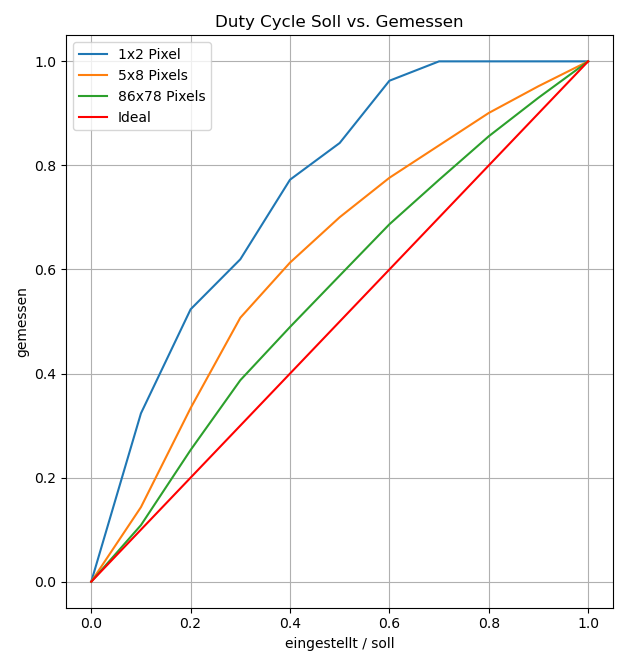
\includegraphics[width=\linewidth]{../images/pwm-test.png}
    \vspace{-2.5em}
    \captionof{figure}{PWM Machbarkeitsanalyse}
    \label{img:PWM-Machbarkeitsanalyse}

\end{minipage}
\noindent\begin{minipage}[t]{.497\linewidth}\vspace{0pt}

    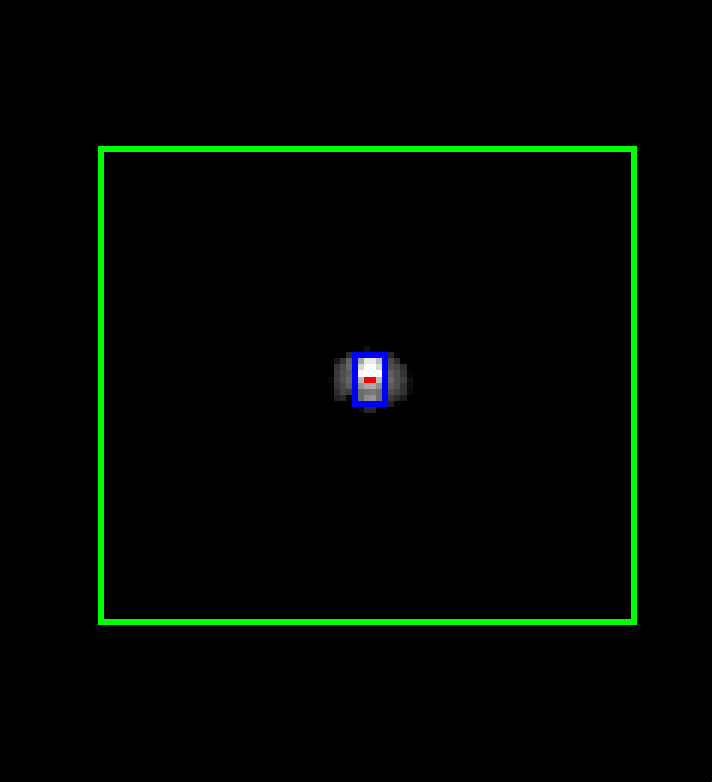
\includegraphics[width=\linewidth]{../images/pwm-test-areas.png}
    \vspace{-2.5em}
    \captionof{figure}{PWM Machbarkeitsanalyse (Ausgewertete Flächen)}
    \label{img:PWM-Machbarkeitsanalyse-Flächen}

\end{minipage}

\subsubsection{Überprüfung von Frequenzen}\label{sec:Überprüfung-von-Frequenzen}

% TODO: link oszi
Um die Frequenzen des Messgerätes zu überprüfen wurde ein Oszilloskop verwendet.
Eine Sonde misst direkt an einer LED wie in \imgref{img:Messpunkt-LED} gezeigt,
dessen Ground wie in \imgref{img:Messpunkt-GND} verbunden ist.

\noindent\begin{minipage}[t]{.497\linewidth}\vspace{0pt}
    \begin{centering}
        \includegraphics[width=\linewidth]{../images/phone/messung-frequenzen-d1.jpg}
        \vspace{-2.5em}
        \captionof{figure}{Messpunkt LED}
        \label{img:Messpunkt-LED}
    \end{centering}
\end{minipage}
\noindent\begin{minipage}[t]{.497\linewidth}\vspace{0pt}
    \begin{centering}
        \includegraphics[width=\linewidth]{../images/phone/messung-frequenzen-gnd.jpg}
        \vspace{-2.5em}
        \captionof{figure}{Messpunkt Ground}
        \label{img:Messpunkt-GND}
    \end{centering}
\end{minipage}




\subsubsection{Aufnahme Video}

Diverse Messvideos in verschiedensten Anordnungen können aufgenommen werden.
Bei allen folgenden Messaufbauten ist die automatische Positionserkennung und Auswertung möglich.

Zum Beginn werden alle LEDs ausgeschaltet über den \hyperlinkXY{hyp:mode-none} Modus und die Zielfrequenz des Messgeräts über die Konfiguration \hyperlinkXY{hyp:config-fps} eingestellt.
Danach wird die Aufnahme und der \hyperlinkXY{hyp:mode-auto} Modus gestartet.
Die Kamera und das Messgerät werden während der gesamten Aufnahmezeit nicht verschoben.
Ausserdem sollte sich die Umgebungshelligkeit so wenig wie möglich ändern, damit die Zuverlässigkeit der Ergebnisse erhöht werden kann.

Zur optimalen Objektiveinstellung und Überprüfung, ob das gesamte LED-Feld im Video sichtbar ist,
empfiehlt es sich alle LEDs vor der obig beschriebenen Aufnahme leuchten lassen um dies zu kontrollieren.
%
Der Code in \appref{app:camera-control} zeigt, wie dieser gesamte Prozess von Konfiguration zur Aufnahme automatisiert werden kann.

\tablevspaceASenum
\begin{longtable}[l]{ @{} >{\RaggedRight\hspace{0pt}} lp{.96\linewidth} @{} }
    \textbullet & Die Möglichkeit in \imgref{img:Aufbau-Normal} zeigt die kontrollierte fixierung der Kamera welche normal auf das Gerät schaut. \\
    \textbullet & In \imgref{img:Aufbau-Weit-Normal} ist dieselbe Kamera ungefähr fünf Meter entfernt beschwert und positioniert worden. Das Gerät ist noch zusätzlich rotiert aufgestellt. \\
    \textbullet & Bei \imgref{img:Aufbau-Weit-Schräg} ist die Kamera ungefähr zwei Meter entfernt positioniert und das Gerät ist noch zusätzlich rotiert und schräg aufgestellt. \\
    \textbullet & Bei \imgref{img:Aufbau-Nah-Schräg} ist die Kamera so nah wie möglich positioniert, sodass das Gerät gerade noch sichtbar ist im Video. Das Gerät ist noch zusätzlich rotiert und schräg aufgestellt. \\
    \addtocounter{table}{-1}\setcounter{enumi}{0}
\end{longtable}


\noindent\begin{minipage}[t]{\dimexpr.994\linewidth/3}\vspace{0pt}
    \begin{centering}
        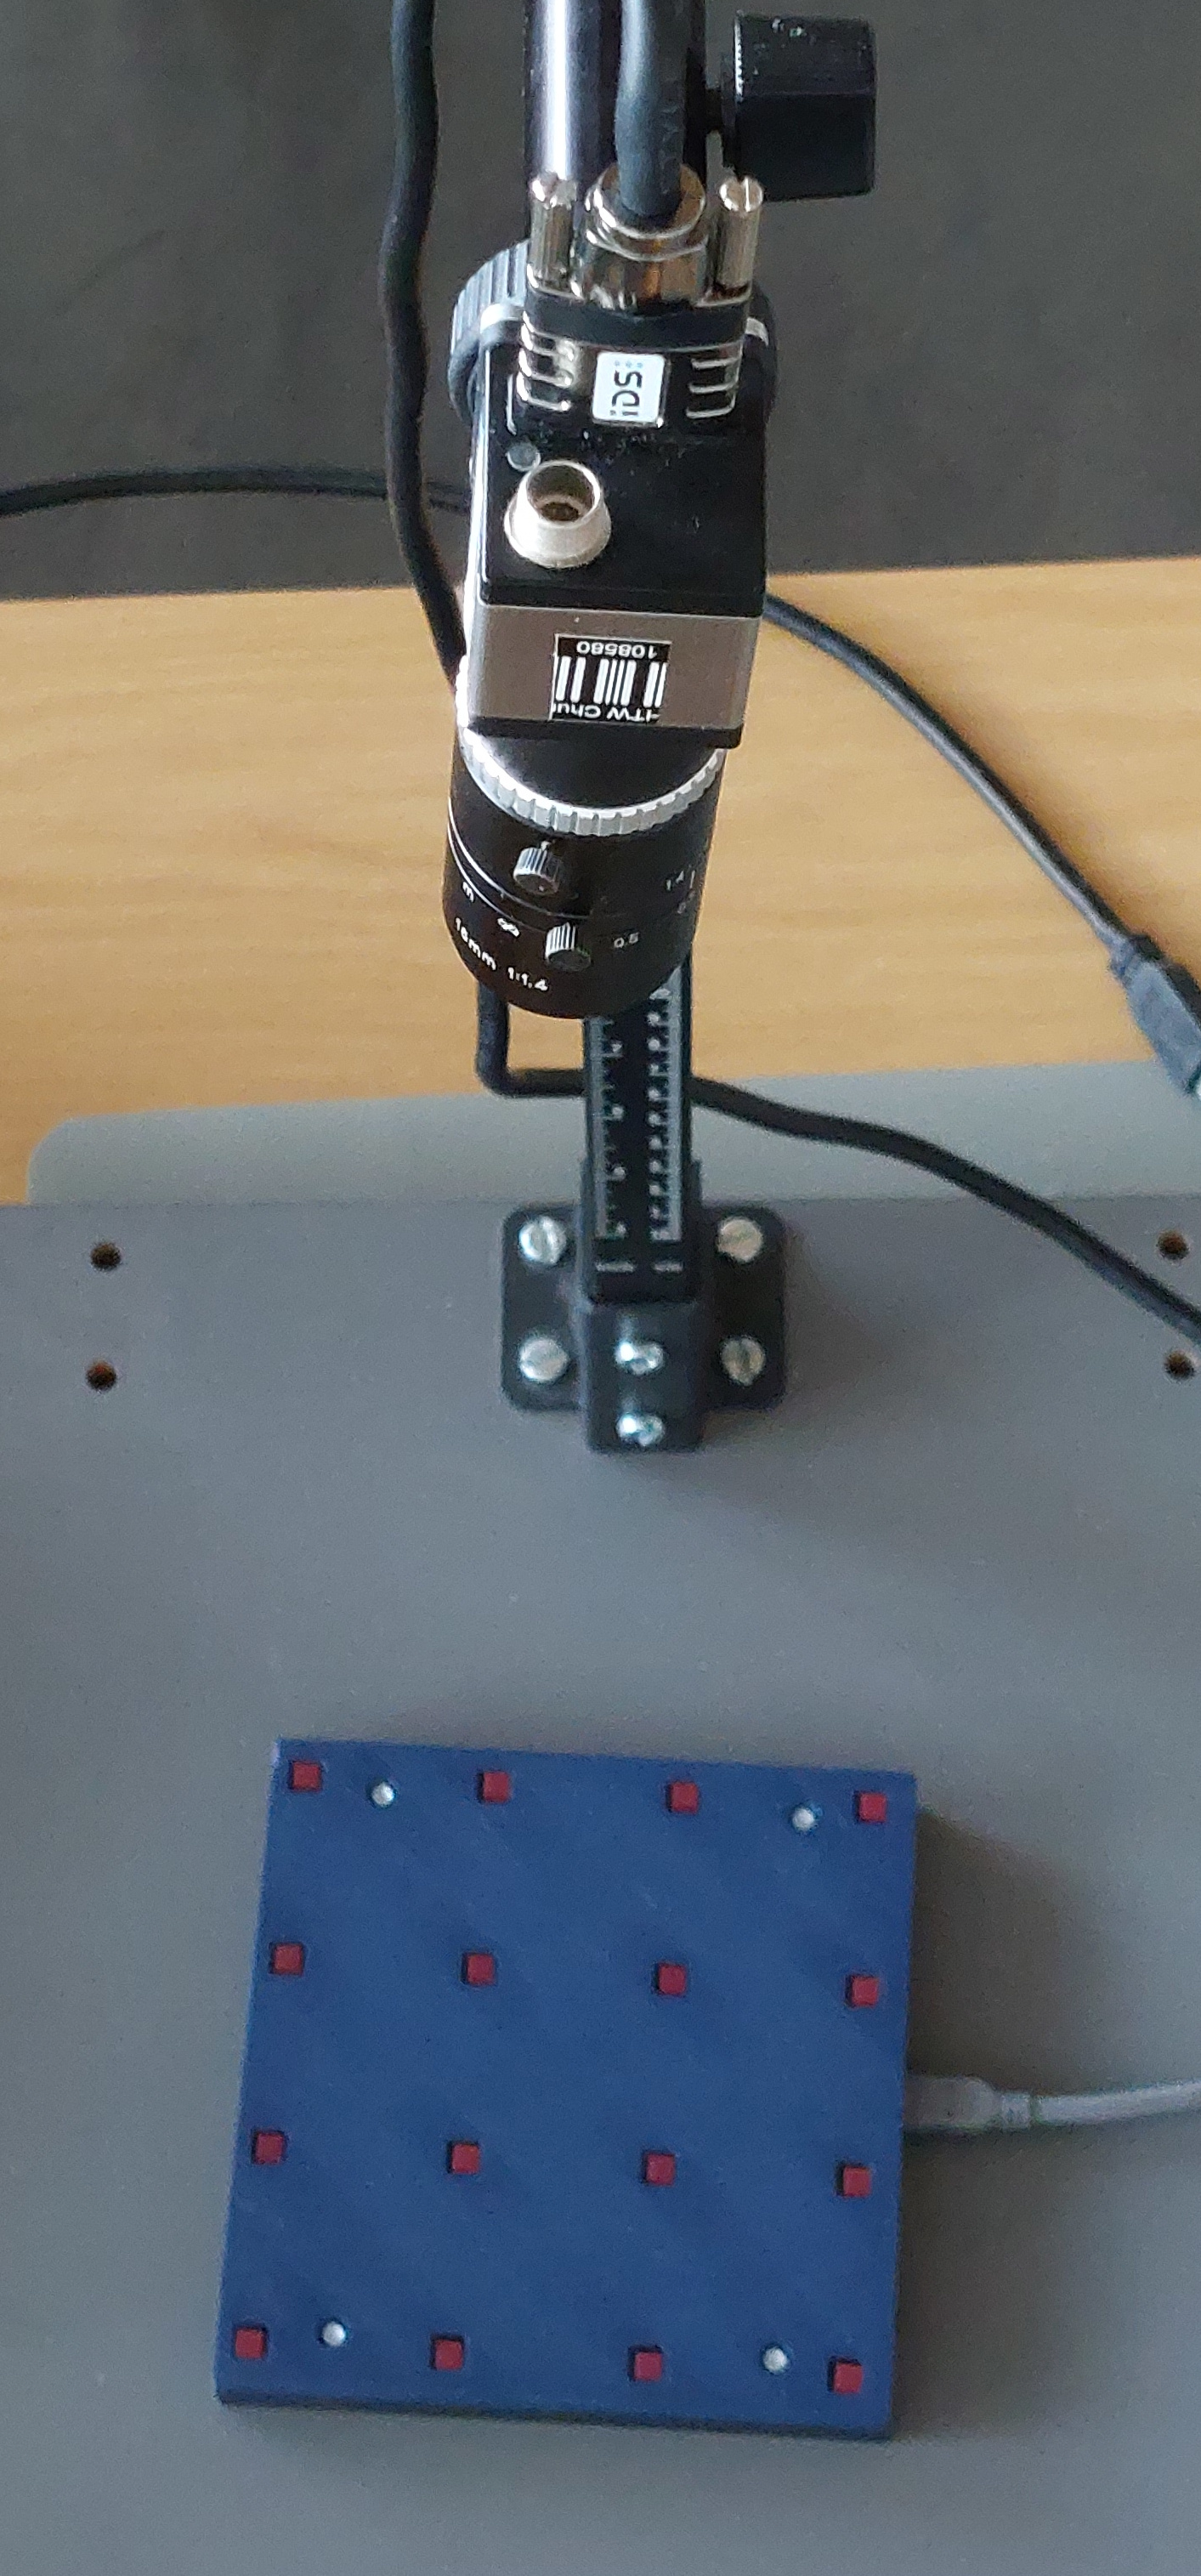
\includegraphics[height=30em]{../images/phone/aufbau-normal-cut.jpg}
        \vspace{-1.0em}
        \captionof{figure}{Aufbau Aufnahme}
        \label{img:Aufbau-Normal}
    \end{centering}
\end{minipage}
\noindent\begin{minipage}[t]{\dimexpr.994\linewidth/3}\vspace{0pt}
    \begin{centering}
        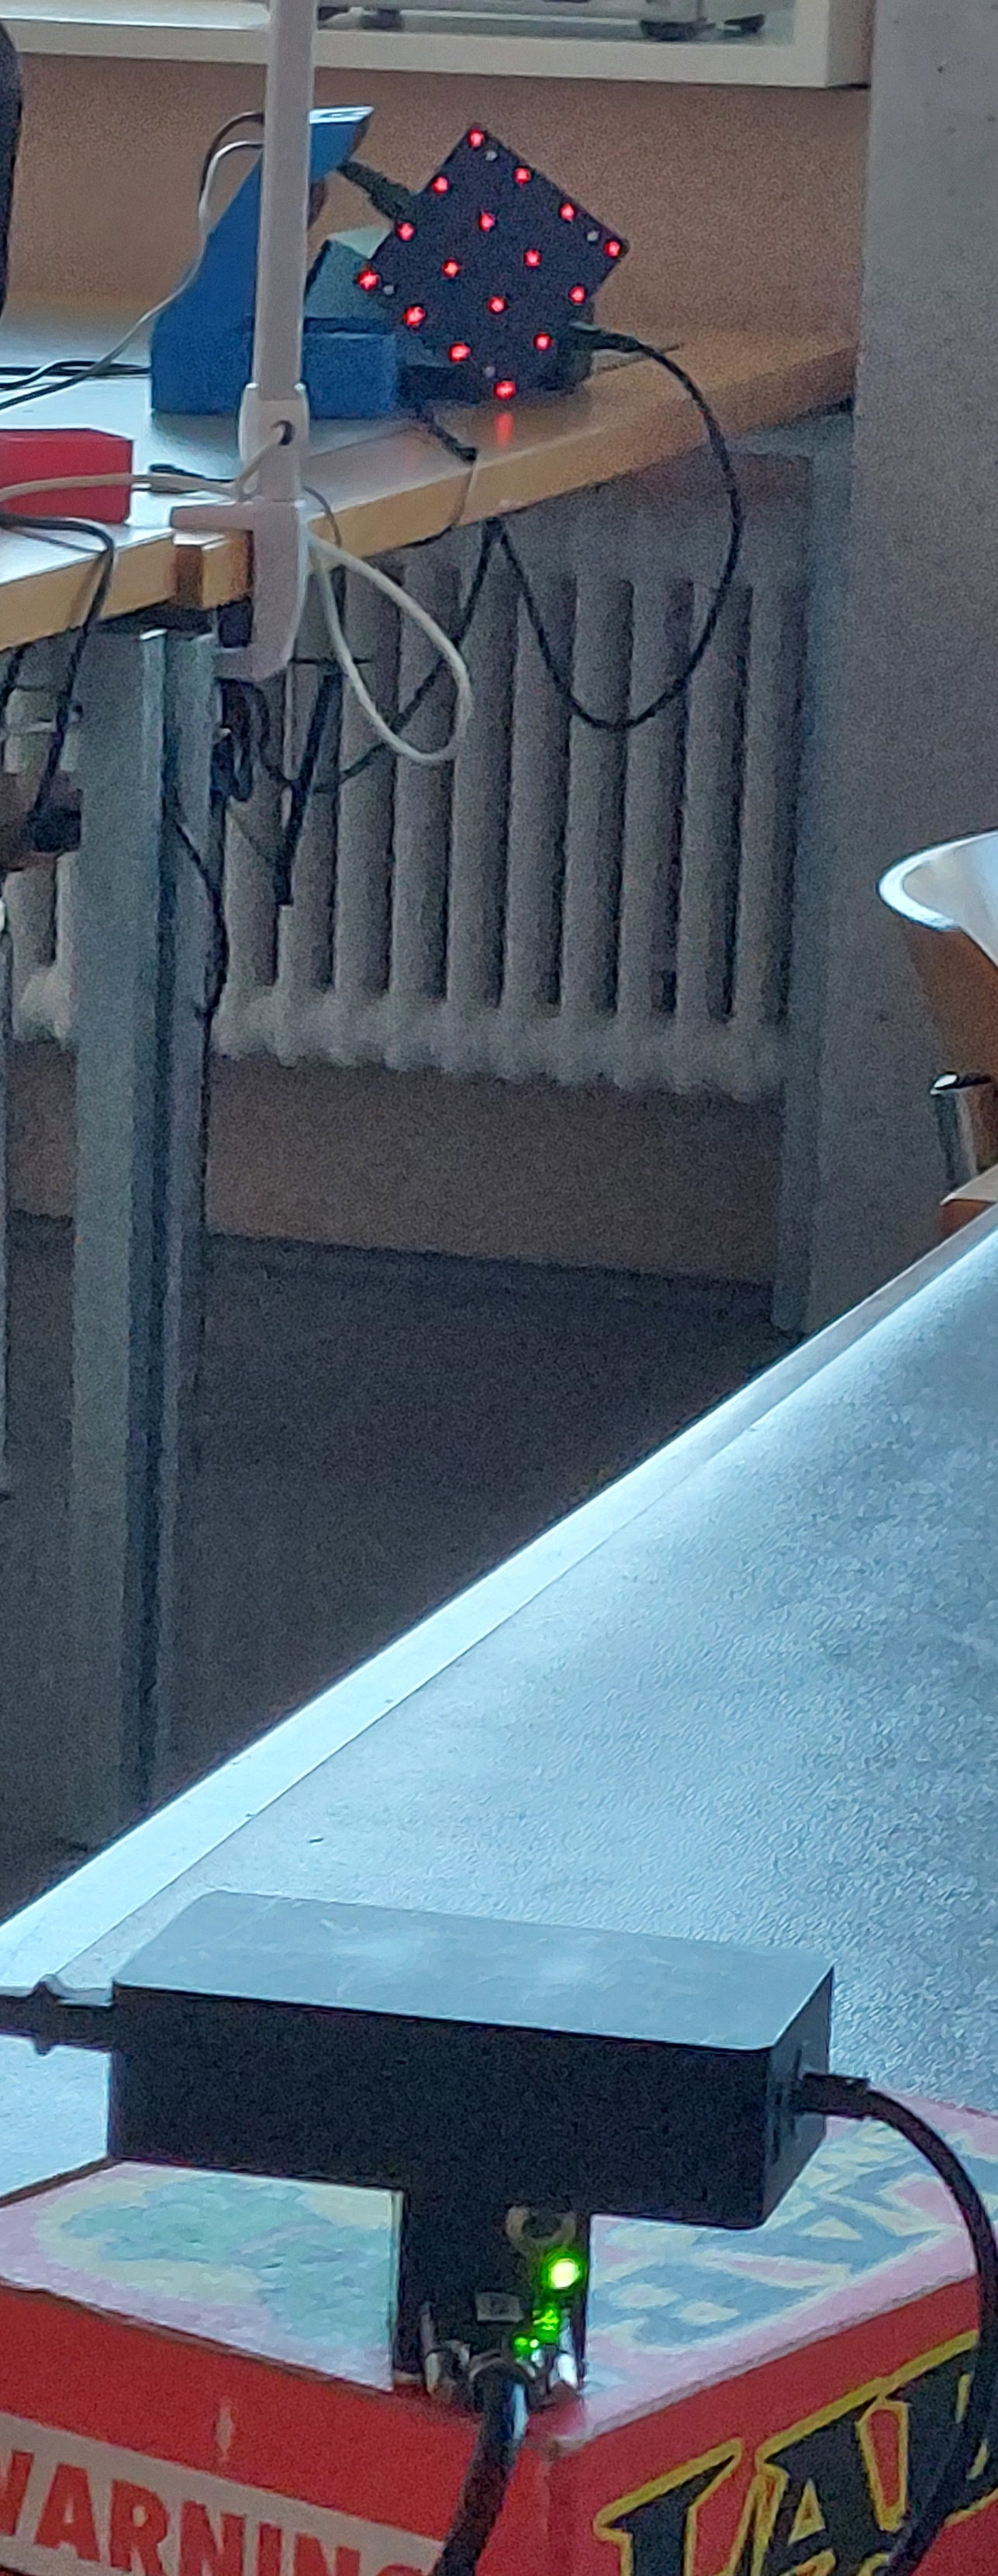
\includegraphics[height=30em]{../images/phone/aufbau-weit-normal-cut.jpg}
        \vspace{-1.0em}
        \captionof{figure}{Aufbau (Weit)}
        \label{img:Aufbau-Weit-Normal}
    \end{centering}
\end{minipage}
\noindent\begin{minipage}[t]{\dimexpr.994\linewidth/3}\vspace{0pt}
    \begin{centering}
        \includegraphics[height=30em]{../images/phone/aufbau-weit-schräg-cut.jpg}
        \vspace{-1.0em}
        \captionof{figure}{Aufbau (Weit + Schräg)}
        \label{img:Aufbau-Weit-Schräg}
    \end{centering}
\end{minipage}

    \includegraphics[width=\linewidth]{../images/phone/aufbau-nah-schräg-cut.jpg}
    \vspace{-2.5em}
    \captionof{figure}{Aufbau (Nah + Schräg)}
    \label{img:Aufbau-Nah-Schräg}


%}}}

\subsection{Auswerteverfahren}\label{sec:Auswerteverfahren} %{{{

%}}}

\subsubsection{Reihenfolge der Modi}\label{sec:Reihenfolge-der-Modi} %{{{

Die Reihenfolge der Modi im \hyperlinkXY{hyp:mode-auto} Modus ist in \tabref{table:Reihenfolge-der-Modi} beschrieben.

\tablevspaceAStable
\begin{tabular}{ @{} >{\RaggedRight\hspace{0pt}} lllll @{} }
    \# & Schritt & \hyperlink{sec:Modi}{Modus} & Beschreibung & Zweck \\
    \hline
    \hypertarget{order:step1}{1.}   & \verb|ALL_OFF| & \hyperlinkXY{hyp:mode-none} & Alle LEDs aus & Initiale Detektion \\
    \hypertarget{order:step2}{2.}   & \verb|ALL_ON| & \hyperlinkXY{hyp:mode-display} & Alle LEDs ein & Initiale Detektion \\
    \hypertarget{order:step3}{3.}   & \verb|PATTERN| & \hyperlinkXY{hyp:mode-display} & Orientierungsmuster & Initiale Detektion \\
    \hypertarget{order:step4}{4.}   & \verb|SYS_FREQ| & \hyperlinkXY{hyp:mode-display} & Systemfrequenz in MHz & Übermittlung Einstellungen \\ % ABBREV
    \hypertarget{order:step5}{5.}   & \verb|PSC| & \hyperlinkXY{hyp:mode-display} & Prescaler vom Timer & Übermittlung Einstellungen \\
    \hypertarget{order:step6}{6.}   & \verb|ARR| & \hyperlinkXY{hyp:mode-display} & Auto-Reload-Register vom Timer & Übermittlung Einstellungen \\
    \hypertarget{order:step7}{7.}   & \verb|PWM_COUNT| & \hyperlinkXY{hyp:mode-display} & Anzahl von PWM Stufen & Kalibration für Rider \\ % ABBREV
    \hypertarget{order:step8}{8.}   & \verb|PWM_CYCLE| & \hyperlinkXY{hyp:mode-pwm} & PWM Stufen & Kalibration für Rider \\ % ABBREV
    \hypertarget{order:step9}{9.}   & \verb|PWM_END| & \hyperlinkXY{hyp:mode-none} & Alle LEDs aus & Kalibration für Rider \\
    \hypertarget{order:step10}{10.} & \verb|RIDER| & \hyperlinkXY{hyp:mode-rider} & Eine LED wandert kontinuierlich & Tatsächliche Auswertung \\
\end{tabular}
\captionof{table}{Reihenfolge der Modi}
\label{table:Reihenfolge-der-Modi}
%}}}

\subsubsection{Detektion \& Ausrichtung des Orientierungsmuster}\label{sec:Detektion-Ausrichtung-des-Orientierungsmuster} %{{{

Hierfür werden die ersten drei Schritte \hyperlink{order:step1}{\texttt{ALL\_OFF}}, \hyperlink{order:step2}{\texttt{ALL\_ON}} \& \hyperlink{order:step3}{\texttt{PATTERN}} verwendet.

\aparagraph{Detektion aller LEDs \& Finden des Orientierungsmuster}

In diesem ersten Schritt werden ein aktuelles Bild mit dem vorangehenden verglichen.
Auschlaggebender Indikator für eine Musteränderung ist ein globaler Unterschied der Pixelhelligkeiten.
Die zwei Schritte, welche darauf zurückgreifen, sind in \tabref{table:Initiale-Detektion} aufgelistet.

\tablevspaceAStable
\begin{tabular}{ @{} >{\RaggedRight\hspace{0pt}} llll @{} }
  Vorherig & Aktuell & Indikator & Gewonnene Information\\
  \hline
  \hyperlink{order:step1}{\texttt{ALL\_OFF}} & \hyperlink{order:step2}{\texttt{ALL\_ON}} & Alle LEDs beginnen zu leuchten & Index $i_{\texttt{ALL\_ON}\bot}$ des Schrittes im Video \\
  \hyperlink{order:step2}{\texttt{ALL\_ON}} & \hyperlink{order:step3}{\texttt{PATTERN}} & Mehrere LEDs schalten aus & Index $i_{\texttt{PATTERN}\bot}$ des Schrittes im Video \\
\end{tabular}
\captionof{table}{Initiale Detektion}
\label{table:Initiale-Detektion}
\tablevspaceAStable

Aus den nun bekannten Indizes können robust
$i_\texttt{ALL\_OFF}$ \eqref{eq:i_ALL_OFF},
$i_\texttt{ALL\_ON}$ \eqref{eq:i_ALL_ON} und
$i_\texttt{PATTERN}$ \eqref{eq:i_PATTERN}
berechnet werden, in denen jeweils keine, alle LEDs, oder das Orientierungsmuster zu sehen sind im Bild \eqref{eq:M_i}.

\begin{equation}\label{eq:i_ALL_OFF}
  i_\texttt{ALL\_OFF} = \left\lfloor \frac{3\cdot i_{\texttt{ALL\_ON}\bot} - i_{\texttt{PATTERN}\bot}}{2} \right\rceil
\end{equation}

\begin{equation}\label{eq:i_ALL_ON}
  i_\texttt{ALL\_ON} = \left\lfloor \frac{i_{\texttt{PATTERN}\bot} + i_{\texttt{ALL\_ON}\bot}}{2} \right\rceil
\end{equation}

\begin{equation}\label{eq:i_PATTERN}
  i_\texttt{PATTERN} = \left\lfloor \frac{3\cdot i_{\texttt{PATTERN}\bot} - i_{\texttt{ALL\_ON}\bot}}{2} \right\rceil
\end{equation}

\begin{equation}\label{eq:M_i}
    M_i = \text{Bild Nummer ''} i \text{`` im Video}
\end{equation}

%}}}

\aparagraph{Gültige Positionen Filtern}\label{sec:Gültige-Positionen-Filtern} %{{{

Hierfür werden die beiden Bilder \img{Dunkel} und \img{Hell}, bei jeweils den indizes \eqref{eq:i_ALL_OFF} und \eqref{eq:i_ALL_ON}, verwendet.

Nacheinander kommen folgende Schritte zur Anwendung, um möglichst robust die gültige Position $p$ des Gerätes zu finden:

\tablevspaceASenum
\begin{longtable}[l]{ @{} >{\RaggedRight\hspace{0pt}} lp{.9\linewidth} @{} }
    \refstepcounter{enumi}\theenumi. & Berechnung von $\img{Unterschied} = \img{Dunkel} - \img{Hell}$
    \\\refstepcounter{enumi}\theenumi. & Anwenden von OTSU-Filter \cite{opencv-threshold} auf \img{Unterschied}
    \\\refstepcounter{enumi}\theenumi. & Konturen finden \& deren Zentren berechnen
    \\\refstepcounter{enumi}\theenumi. & Alle Zentren verbinden \& deren Längen berechnen
    \\\refstepcounter{enumi}\theenumi. & Winkel der Verbindungen berechnen und ähnlich orientierte Verbindungen gruppieren
    \\\refstepcounter{enumi}\theenumi. & Gruppierung mit den meisten Winkeln ergibt die Hauptrichtung
    \\\refstepcounter{enumi}\theenumi. & Gruppierung mit genügend grosser Winkeldifferenz zur Hauptrichtung ergibt die zweite Richtung
    \\\refstepcounter{enumi}\theenumi. & Verbindungen ziehen entlang der ersten und zweiten Richtung
    \\\refstepcounter{enumi}\theenumi. & Die kürzesten acht Verbindungen verwerfen in beiden Richtungen (um zum Beispiel Spigelungen an einem Tisch herauszufiltern)
    \\\refstepcounter{enumi}\theenumi. & Lange Verbindungen verwerfen in beiden Richtungen
    \\\refstepcounter{enumi}\theenumi. & Verbleibenden Verbindungen welche nicht auf jeweils mindestens zwei Konturen fallen verwerfen
    \\\refstepcounter{enumi}\theenumi. & Finale Verbindungen gehen zurück auf die Zentren der Konturen, dies sind die Positionen
    \\\refstepcounter{enumi}\theenumi. & Finale Positionen in X- und Y-Richtung sortieren 
    \addtocounter{table}{-1}\setcounter{enumi}{0}
\end{longtable}

%\tablevspaceASenum

% abzug hell-dunkel => otsu threshold
% konturen finden
% zentren der konturen finden
% alle zentren verbinden
% kürzeste 8 strecken streichen
% ähnliche winkel gruppieren -> 1. und 2. orientierung -> diese linien beibehalten
% nun nur die linien beibehalten, die innerhalb eines vier-eck eines anderen punkes sind
% sortieren der punkte nach x- und y- richtung

% Feedback: Bilder aus der Präsentation ebenfalls hier einfügen :)

%}}}

\aparagraph{Interpretation des Orientierungsmuster}\label{sec:Interpretation-des-Orientierungsmuster} %{{{

Das zu untersuchende Bild, welches das Orientierungsmuster anzeigt, ist durch \eqref{eq:i_PATTERN} gegeben.
Ausserdem wird, ähnlich zum vorherigen Schritt ein ``Dunkel''-Bild \eqref{eq:i_ALL_OFF} abgezogen vom zu untersuchenden Bild.

\begin{equation}\label{eq:hat-M_PATTERN}
  \widehat{M}_{\texttt{PATTERN}} = \frac{M_{\texttt{PATTERN}} - M_{\texttt{ALL\_OFF}} }{M_{\texttt{ALL\_ON}} - M_{\texttt{ALL\_OFF}} }
\end{equation}

Die normierten Zustände der LEDs werden in \eqref{eq:hat-M_PATTERN} bei den vorherig ermittelten Positionen bestimmt.
In einem vom Benutzer beeinflussten Radius wird für jede Position der Mittelwert gebildet.
Durch binäres Thresholding um 0.5 werden die Bit-Zustände berechnet.

\noindent\begin{minipage}[t]{.65\linewidth}\vspace{0pt}
\vspace{-0.65em}
  Das Gerät zeigt die Hexadezimalzahl \texttt{0x842F} als Orientierungsmuster an.
  Auf einem 4x4 Bitfeld resultiert dies in einem ``Pfeil'', welcher auf das LSB (Least significant Bit) zeigt, wie in \tabref{table:Orientierungsmuster} zu sehen.

  Das gezeigte Muster kann gespiegelt oder eine beliebige Richtung gedreht sein.
  Um das Muster korrekt zu orientieren, wird im ersten Schritt die Reihe gesucht, in der alle vier Bits aktiv sind (rot dargestellt).

\end{minipage}
\noindent\begin{minipage}[t]{.33\linewidth}\vspace{0pt}
  \begin{center}
    \begin{tabular}{ | >{\RaggedRight\hspace{0pt}} c|c | }
      \hline \text{Muster} & \text{Gespiegelt} \\\hline
      \begin{tabular}{ @{} >{\RaggedRight\hspace{0pt}} c @{} }
        \texttt{1 0 0 0} \\
        \texttt{0 1 0 0} \\
        \texttt{0 0 1 0} \\
        \texttt{\textbf{\color{red}1 1 1 1}} \\
      \end{tabular}
      &
      \begin{tabular}{ @{} >{\RaggedRight\hspace{0pt}} c @{} }
        \texttt{\textbf{\color{blue}0} 0 0 1} \\
        \texttt{\textbf{\color{blue}0} 0 1 0} \\
        \texttt{\textbf{\color{blue}0} 1 0 0} \\
        \texttt{\textbf{\color{blue}1} 1 1 1} \\
      \end{tabular}
      \\\hline
    \end{tabular}
    \captionof{table}{Orientierungsmuster}
    \label{table:Orientierungsmuster}
  \end{center}
  \setlength\lineskip{0pt}
\end{minipage}

\strut Danach kann das Muster um 90° gedreht nach den Reihenfolgen \texttt{0b1000} (blau dargestellt), \texttt{0b1100}, \texttt{0b1010} und \texttt{0b1001} überprüft werden.

% }}}

\subsubsection{Übermitteln von Einstellungen \& Kalibration der Leuchtdioden-Intensität} %{{{

Es werden die Schritte \hyperlink{order:step4}{\texttt{SYS\_FREQ}}, \hyperlink{order:step5}{\texttt{PSC}}, \hyperlink{order:step6}{\texttt{ARR}}, \hyperlink{order:step7}{\texttt{PWM\_COUNT}}, \hyperlink{order:step8}{\texttt{PWM\_CYCLE}} \& \hyperlink{order:step9}{\texttt{PWM\_END}} analysiert.

\aparagraph{Erkennen aller Binärwerte}\label{sec:Erkennen-aller-Binärwerte}

Bild für Bild wird die Binärzahl ausgewertet des aktuellen Bildes $M_\textit{aktuell}$ bei index $i_\textit{aktuell}$ in \eqref{eq:hat-M_aktuell}.

\begin{equation}\label{eq:hat-M_aktuell}
  \widehat{M}_{\textit{aktuell}} = \frac{M_{\textit{aktuell}} - M_{\texttt{ALL\_OFF}} }{M_{\texttt{ALL\_ON}} - M_{\texttt{ALL\_OFF}} }
\end{equation}

Die zu erwartenden Werte sind alle unbekannt aber grösser als $0$.
Einzig der Wert nach dem Anzeigen von allen digitalen Informationen, bei der PWM-Stufe 0\% ist bekannt, nämlich $0$.
Ausschlaggebender Index ist folglich $i_{\texttt{PWM\_0\%}\bot}$ wenn eine $0$ angezeigt wird.
Dazu wird der Unterschied in \eqref{eq:Delta_i} gebraucht, um
die restlichen Indizes der Schritte \hyperlinkXY{order:step4} \eqref{eq:i_SYS_FREQ} bis \hyperlinkXY{order:step7} \eqref{eq:i_PWM_COUNT} zu ermitteln.

\begin{align}
  % https://tex.stackexchange.com/questions/44450/how-to-align-a-set-of-multiline-equations
  \phantom{i_{\texttt{PWM\_COUNT}} } % längste linke Hälfte
    &\begin{aligned}\label{eq:Delta_i}
    \mathllap{ \Delta i} &= \frac{i_{\texttt{PWM\_0\%}\bot} - i_{\texttt{PATTERN}\bot}}{5}
  \end{aligned}\\
    &\begin{aligned}\label{eq:i_SYS_FREQ}
    \mathllap{ i_{\texttt{SYS\_FREQ}} } &= i_{\texttt{PATTERN}\bot} + \frac{3 \cdot \Delta i}{2}
  \end{aligned}\\
  &\begin{aligned}
    \mathllap{ i_{\texttt{ARR}} } &= i_{\texttt{PATTERN}\bot} + \frac{5 \cdot \Delta i}{2}
  \end{aligned}\\
  &\begin{aligned}
    \mathllap{ i_{\texttt{PSC}} } &= i_{\texttt{PATTERN}\bot} + \frac{7 \cdot \Delta i}{2}
  \end{aligned}\\
  &\begin{aligned}\label{eq:i_PWM_COUNT}
    \mathllap{ i_{\texttt{PWM\_COUNT}} } &= i_{\texttt{PATTERN}\bot} + \frac{9 \cdot \Delta i}{2}
  \end{aligned}
  %\end{equation}
\end{align}

Um die Robustheit sicherzustellen, wird bei jedem Index jeweils um $\pm \frac{\Delta i}{4}$ erweitert in \eqref{eq:M_i_Delta_i} und die angezeigten Binärzahlen der entsprechenden Bilder ausgewertet.

\begin{equation}\label{eq:M_i_Delta_i}
  \bar{M}_i(\Delta i) = \left\lfloor \frac{2}{\Delta i} \right\rceil \sum_{ k=\left\lfloor i-\frac{\Delta i}{4} \right\rceil }^{ \left\lfloor i+\frac{\Delta i}{4} \right\rceil } \widehat{M}_{k}
\end{equation}


\aparagraph{Intensitätskalibration}

Die Intensitätskalibration (siehe \secref{sec:Machbarkeitsanalyse-der-Kalibration}) geschieht über die PWM Ansteuerung der LEDs.

Ähnlich wie im \secref{sec:Erkennen-aller-Binärwerte} wird zuerst das Ende von \hyperlink{order:step9}{\texttt{PWM\_END}} $i_{\texttt{PWM\_END}\bot}$ gesucht, wo alle LEDs ausgeschaltet sind.
Die Anzahl an PWM-Stufen in linearen Abständen ist vorgegeben durch \eqref{eq:i_PWM_COUNT}.
Durch die Anzahl an Stufen und den Start- \& Stopp-Indizes $i_{\texttt{PWM\_0\%}\bot}$ und $i_{\texttt{PWM\_END}\bot}$ werden die Helligkeiten bestimmt und für zukünftige Messungen linear interpoliert
in \eqref{eq:Delta_i_PWM}.

\begin{equation}\label{eq:Delta_i_PWM}
  \Delta i_\texttt{PWM} = \frac{i_{\texttt{PWM\_END}\bot} - i_{\texttt{PWM\_0\%}\bot} }{n_{\texttt{PWM\_COUNT}} + 1 }
\end{equation}

Die Bilder bei PWM-Stufen $k\in\{\,0 \ldots n_\texttt{PWM\_COUNT}\,\}$ in \eqref{eq:i_PWM_k} werden mithilfe von \eqref{eq:M_i_Delta_i} über \eqref{eq:Delta_i_PWM} gemittelt. Bei den Positionen $p$ werden in \eqref{eq:hat_M_PWM_k_Delta_i_PWM} die Helligkeiten ausgewertet.

\begin{equation}\label{eq:i_PWM_k}
  i_{\texttt{PWM}}(k) = k\cdot \Delta i_\texttt{PWM} + i_{\texttt{PWM\_0\%}} + \frac{\Delta i_\texttt{PWM}}{2}
\end{equation}

\begin{equation}\label{eq:hat_M_PWM_k_Delta_i_PWM}
  \bar{M}_\texttt{PWM}(k)(\Delta i_\texttt{PWM})
\end{equation}

Angenommen das Gerät ist konfiguriert auf 16 PWM-Stufen, so sind die Helligkeiten von 0\% bis 100\% in 16 Schritten linear abgebildet.
In \imgref{img:PWM-Kurven-bei-offener-Blende} und \imgref{img:PWM-Kurven-bei-mittlerer-Blende} sind die Punkte die gemessenen Helligkeiten und die gestrichelten Linien die rückwärts linear interpolierten Kurven.

\vspace{-1em}
\noindent\begin{minipage}[t]{.49\linewidth}\vspace{0pt}
  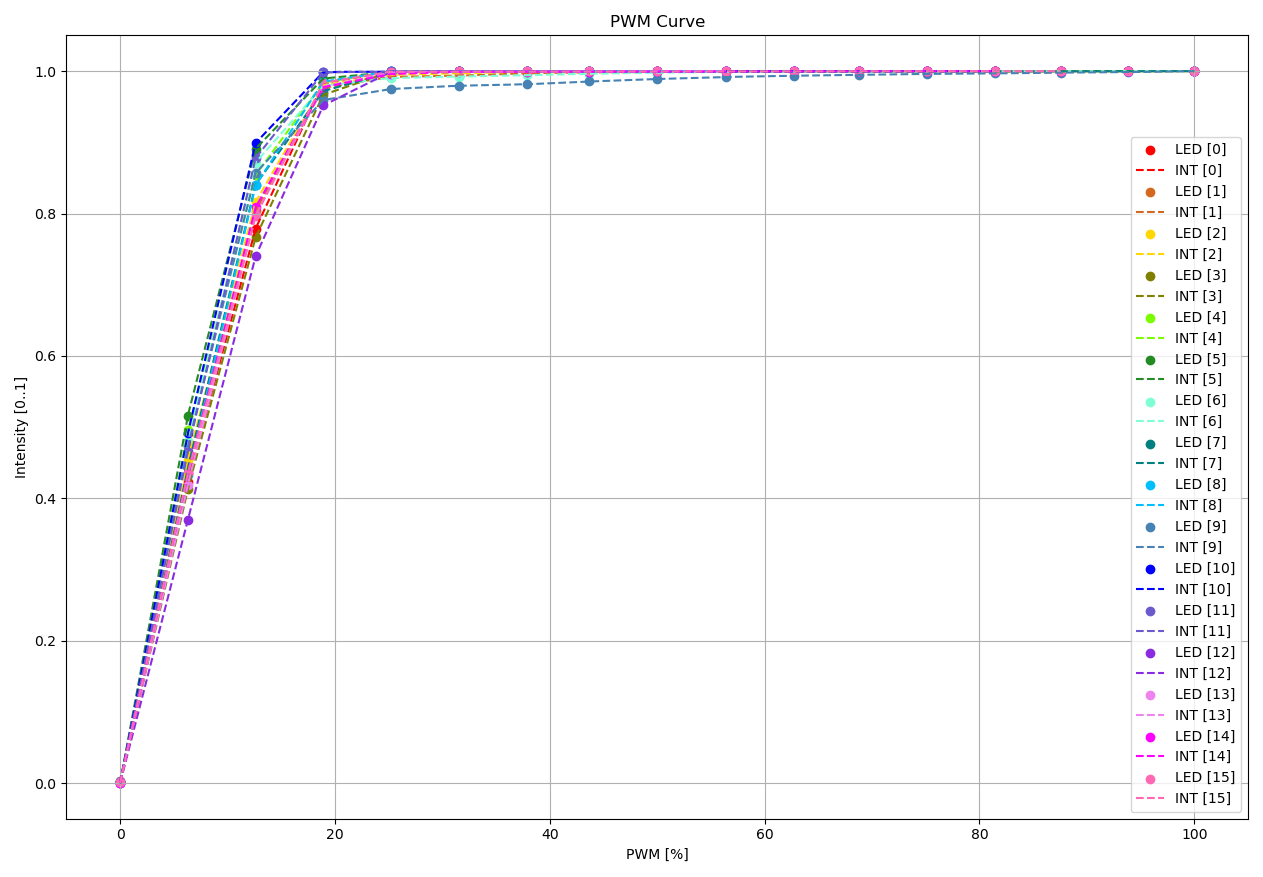
\includegraphics[width=\linewidth]{../images/pwm-curves/30fps-4999us-at-29.85fps-PWM.png}
  \vspace{-2.5em}
  \captionof{figure}{PWM Kurven bei offener Blende}
  \label{img:PWM-Kurven-bei-offener-Blende}
\end{minipage}
\noindent\begin{minipage}[t]{.49\linewidth}\vspace{0pt}
  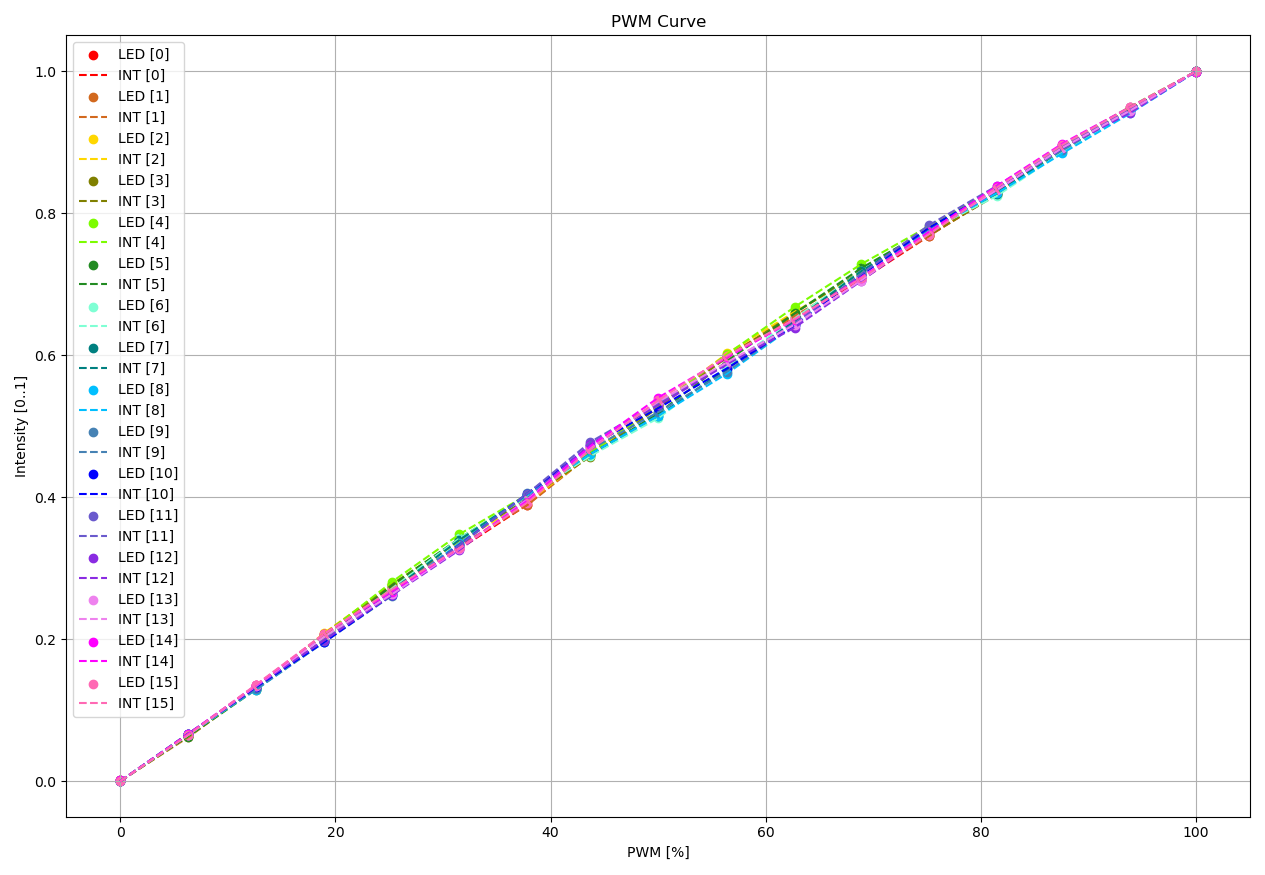
\includegraphics[width=\linewidth]{../images/pwm-curves/59.99fps-4999us-at-60.299084fps-PWM.png}
  \vspace{-2.5em}
  \captionof{figure}{PWM Kurven bei mittlerer Blende}
  \label{img:PWM-Kurven-bei-mittlerer-Blende}
\end{minipage}

%}}}

\subsubsection{Zentrum der laufenden Leuchtdiode}\label{sec:Zentrum-def-laufenden-Leuchtdiode} %{{{

% TODO: beispielbild? => zeigen dass mehr als eine LED leuchtet

Das Zentrum der aktiven Leuchtdioden wird als Kodierung der Stabilität im Video verwendet.
Für den Fall, wenn die aktiven LEDs beide Ränder überlappen, muss dies berücksichtigt werden.
%
Der gewählte Ansatz \eqref{eq:varphi} ordnet die LEDs in der Berechnung im Kreis an und berechnet aus den Intensitäten $I$ den Winkel $\varphi$.
%
So ist auch im Fall, wenn eine Wanderung vom einen Rand zum anderen geschieht, klar in welche Richtung sich diese bewegt.

\begin{equation}\label{eq:varphi}
    \varphi = \arctan \left(
    \sum_{k=0}^{n_\text{LED}-1} \frac{
        \sin\left( \frac{2\pi k I_{k+1}}{n_\text{LED}} \right) }{
        \cos\left( \frac{2\pi k I_{k+1}}{n_\text{LED}} \right) }
    \right)
\end{equation}

Über den Prescaler und Auto-Reload ist $f_R$ durch \eqref{eq:f_Timer} gegeben.
Durch diverse Toleranzen der elektronischen Bauteile ist die eingestellte Geschwindigkeit $f_R$ der LEDs ungleich der reellen $f_G$, siehe \secref{sec:Rider-Modus}.
Es ist wichtig, dass eine korrekte Einstellung der Frequenz vom Messgerät vorgenommen wird, siehe \secref{sec:Gut-Eingestellt}.

Der Unterschied der Eingestellten tatsächlichen Frequenz $f_G$ zur Kamerafrequenz ist durch \eqref{eq:Delta-f} gegeben.
Daraus und mit \eqref{eq:varphi} lässt sich ein Unterschied in Winkeländerungen $\Delta\dot\varphi$ \eqref{eq:Delta-dot-varphi} berechnen.
Dieser Unterschied korreliert mit der Abweichung von der eingestellten zur ermittelten Kamerafrequenz $f$ in \eqref{eq:f}.

\begin{equation}\label{eq:Delta-f}
    \Delta f = f_G - f_K
\end{equation}

\begin{equation}\label{eq:Delta-dot-varphi}
    \Delta \dot\varphi = 2\pi\frac{\Delta f}{f_K} - \dot\varphi
\end{equation}

\begin{equation}\label{eq:f}
    f = \frac{2\pi + \frac{\Delta\dot\varphi}{\Delta f}}{2\pi} \cdot f_K
\end{equation}

%}}}


\subsubsection{Breite der laufenden Leuchtdiode}\label{sec:Breite-der-laufenden-Leuchtdiode} %{{{

Aus der Anzahl an aktiven Leuchtdioden über die Intensitäten $I$ und deren maximaler Intensität $I_\text{max}$ wird die Belichtungszeit $b$ im Video ermittelt \eqref{eq:b}.

% TODO: -> die Zeitstempel können nicht absolut, sondern nur relativ bestimmt werden (WIE IN DER EINLEITUNG ERWÄHNT)
% TODO: ... -> ?? Das bestimmen der Belichtungszeit lehnt sich stark an die Kalibration der PWM-Kurven.
% TODO: berechnen nicht mit f_B aber AVG!! von f?!? => sieht es stabiler aus? -> ja

\begin{equation}\label{eq:b}
    b = \frac{1}{\bar f \cdot n_\text{LED}} \sum_{k=1}^{n_\text{LED}} \frac{I_k}{I_\text{max}}
\end{equation}

%}}}

\subsection{Ergebnisse}

\subsubsection{Frequenzlimitationen}

Die maximal Einstellbare Geschwindigkeit einer LED im \hyperlinkXY{hyp:mode-rider} Modus beträgt 4.5kHz.

Die Taktgeschwindigkeit im \hyperlinkXY{hyp:mode-pwm} Modus jeder LED beträgt auch 4.5kHz.


\subsubsection{Frequenzzuverlässigkeit}

\aparagraph{Rider Modus}\label{sec:Rider-Modus}

Verschiedene Frequenzen wurden an einer LED im \hyperlinkXY{hyp:mode-rider} Modus mit einem Oszilloskop gemessen.
In \tabref{table:Eingestellte-Gemessene-Frequenzen} sind die genauen Messwerte aufgelistet und im \appref{app:measurements} beigelegt.
Diese sind in \imgref{img:Eingestellte-Gemessene-Frequenzen} relativ dargestellt und es zeigt sich,
dass
die tatsächliche Frequenz $f_G$ (gelb) bis zu 0.2‰ von der Zielfrequenz $f_R$ abweicht. % und
Die Standardabweichung $\sigma$ (rot) steigt mit der Frequenz.

\noindent\begin{minipage}[t]{.44\linewidth}\vspace{0pt}
\vspace{-1em}
\begin{centering}
\tablevspaceAStable
\begin{tabular}{ @{} >{\RaggedRight\hspace{0pt}} ccc @{} }
    $f_R$ [Hz] & $f_G$ [Hz] & $\sigma$ [µHz] \\
    \hline
    30.000 & 30.005 & 62.566 \\ 
    40.000 & 40.007 & 366.58 \\ 
    56.250 & 56.259 & 129.31 \\ 
    59.700 & 59.711 & 368.78 \\ 
    60.000 & 60.010 & 483.37 \\ 
    60.299 & 60.309 & 425.85 \\ 
    64.286 & 60.309 & 498.19 \\ 
    75.000 & 75.013 & 483.33 \\ 
    120.00 & 120.02 & 1'120.8 \\ 
    284.99 & 285.04 & 3'247.6 \\ 
    752.01 & 752.16 & 20'029 \\
    4500.0 & 4499.6 & 370'780
\end{tabular}
\captionof{table}{Überprüfte Frequenzen}
\label{table:Eingestellte-Gemessene-Frequenzen}
\end{centering}
\end{minipage}
\noindent\begin{minipage}[t]{.55\linewidth}\vspace{0pt}
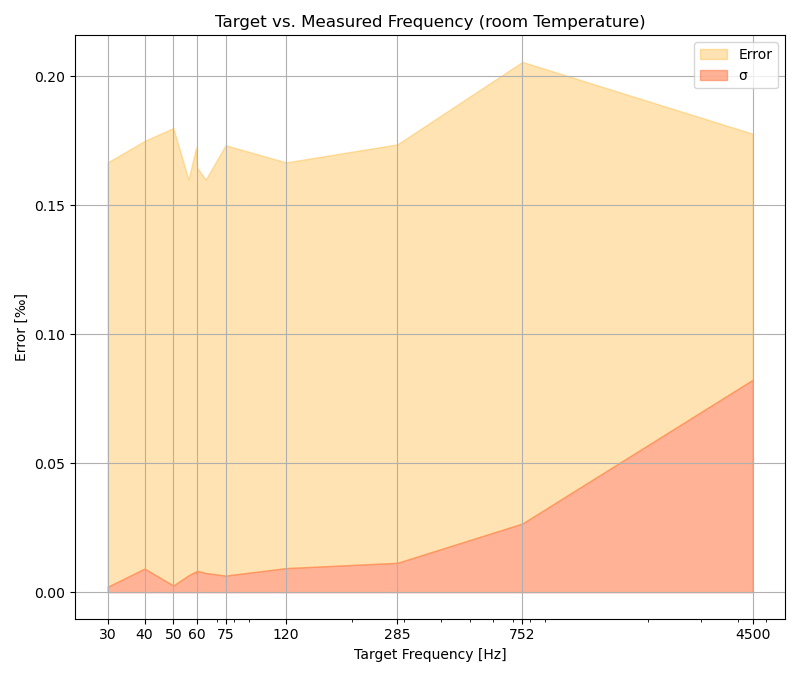
\includegraphics[width=\linewidth]{../images/results-calibrated-frequencies.png}
\vspace{-2.5em}
\captionof{figure}{Überprüfte Frequenzen}
\label{img:Eingestellte-Gemessene-Frequenzen}
\end{minipage}

\aparagraph{PWM Modus}\label{sec:PWM-Modus}

\noindent\begin{minipage}[t]{.52\linewidth}\vspace{0pt}
\vspace{-1em}
\begin{centering}
\tablevspaceAStable
\begin{tabular}{ @{} >{\RaggedRight\hspace{0pt}} cccc @{} }
    $z$ & Eingestellt [\%] & Gemessen [\%] & Fehler [\%] \\
    \hline
    % 6.25 & 6.37 & 1.91 \\ 
    % 50.00 & 50.06 & 0.12 \\ 
    % 93.75 & 93.81 & 0.06 \\
    0 & 0 & 0 & 0.00 \\
    1 & 6.25 & 6.31 & 0.90 \\
    2 & 12.50 & 12.61 & 0.90 \\
    3 & 18.75 & 18.92 & 0.90 \\
    4 & 25.00 & 25.23 & 0.90 \\
    5 & 31.25 & 31.53 & 0.90 \\
    6 & 37.50 & 37.84 & 0.90 \\
    7 & 43.75 & 43.69 & -0.13 \\
    8 & 50.00 & 50.00 & 0.00 \\
    9 & 56.25 & 56.40 & 0.26 \\
    10 & 62.50 & 62.70 & 0.32 \\
    11 & 68.75 & 68.83 & 0.11 \\
    12 & 75.00 & 75.14 & 0.18 \\
    13 & 81.25 & 81.44 & 0.24 \\
    14 & 87.50 & 87.57 & 0.08 \\
    15 & 93.75 & 93.87 & 0.13 \\
    16 & 100.0 & 100.0 & 0.00

\end{tabular}
\captionof{table}{Überprüfte Duty Cycles}
\label{table:Eingestellte-Gemessene-Frequenzen-PWM}
\end{centering}
\end{minipage}
\noindent\begin{minipage}[t]{.47\linewidth}\vspace{0pt}

    Das Messgerät besitzt $n_\texttt{PWM\_COUNT}=16$ PWM-Stufen welche grösser sind als 0\%.
    Der konkrete Duty Cycle $D$ ist gegeben über $z\in\{0\ldots n_\texttt{PWM\_COUNT}\}$ durch \eqref{eq:D}.

    Diese Stufen wurden einzeln an einer LED gemessen worden mit einem Oszilloskop (siehe \secref{sec:Überprüfung-von-Frequenzen}) und in \tabref{table:Eingestellte-Gemessene-Frequenzen-PWM} aufgelistet.
    Alle Messresultate sind im \appref{app:measurements} beigelegt.
    Die Abweichungen werden in der Software (\appref{app:eval-dynamic}) berücksichtigt.

    \begin{equation}\label{eq:D}
        D(z) = 100\%\cdot\frac{z}{n_\texttt{PWM\_COUNT}}
    \end{equation}

\end{minipage}

\aparagraph{Display Modus}

Der \hyperlinkXY{hyp:mode-display} Modus ist nicht zeitkritisch und es wurden deshalb keine Frequenzen überprüft.
Die Aktualisierungs-, bzw. Verzögerungszeit ist unbekannt, denn diese ist im Moment irrelevant.

\subsubsection{Gut eingestellt}\label{sec:Gut-Eingestellt}

Die Frequenz des Messgerätes $f_G$ ist gut eingestellt, wenn sie ein wenig von der Kamerafrequenz $f_K$ abweicht (zum Beispiel ungefähr 0.5\%).
Aus der Differenz der Frequenzen kann die im besten Fall maximal detektierbare Anzahl an ausgelassenen Bildern am Stück $s_\text{maxskip}$ berechnet werden gemäss \eqref{eq:s_maxskip}.

Resultate verschiedener Konfigurationen sind in \tabref{table:Auswertung-Gut} aufgeführt.
Im \appref{app:results} sind detaillierte Grafiken über die Zeit zu allen Resultaten zu finden.
Die Hersteller \cite{ids,aos} geben keine Toleranzen der Kameras an, somit ist kein Vergleich möglich, ob die gemessenen Frequenzen $\bar f$ und Belichtungszeiten $\bar b$ innerhalb einer Toleranz liegen oder nicht.
Dennoch sind die Abweichungen kleiner als 0.3\%, mit einem Ausreisser bei \hyperlinkXY{hyp:k-aos-285}.

\begin{table}[H]
\begin{longtable}[c]{ @{} >{\RaggedRight\hspace{0pt}} lrrrrrl @{} }
    % TODO: länge des clips? median? std?
    Kamera & $f_K$ [Hz] & $f_G$ [Hz] & $\bar f$ [Hz] & $b_K$ [µs] & $\bar b$ [µs] & Bilder in \appref{app:results} % & FPS & Belichtungszeit
    \\ \hline
       \hyperlinkXY{hyp:IDS} & 30.00 & 29.850 & 30.054 & 4999 & 5095 & \hyperlinkXY{hyp:k-ueye-29-85}
    \\ \hyperlinkXY{hyp:IDS} & 59.99 & 58.999 & 59.959 & 4999 & 5123 & \hyperlinkXY{hyp:k-ueye-59}
    \\ \hyperlinkXY{hyp:IDS} & 59.99 & 59.701 & 59.969 & 4999 & 5004 & \hyperlinkXY{hyp:k-ueye-59-7}
    \\ \hyperlinkXY{hyp:IDS} & 59.99 & 60.299 & 59.997 & 4999 & 5063 & \hyperlinkXY{hyp:k-ueye-60-3}
    \\ \hyperlinkXY{hyp:IDS} & 59.99 & 61.000 & 59.978 & 4999 & 5040 & \hyperlinkXY{hyp:k-ueye-61}
    \\ \hyperlinkXY{hyp:AOS} & 60.00 & 58.999 & 59.992 & 5000 & 5021 & \hyperlinkXY{hyp:k-aos-60}
    \\ \hyperlinkXY{hyp:AOS} & 285.0 & 284.99 & 281.70 & 2055 & 1997 & \hyperlinkXY{hyp:k-aos-285}
    \\ \hyperlinkXY{hyp:AOS} & 752.0 & 752.01 & 749.86 &  600 &  512 & \hyperlinkXY{hyp:k-aos-752}
\end{longtable}
\addtocounter{table}{-1}\setcounter{enumi}{0}
\captionof{table}{Auswertung bei gut eingestellten Frequenzen}
\label{table:Auswertung-Gut}
\addtocounter{table}{-1}\setcounter{enumi}{0}
\end{table}

\begin{equation}\label{eq:s_maxskip}
    s_\text{maxskip}=\frac{f_G}{2\cdot|f_G-f_K|}
\end{equation}

\subsubsection{Schlecht eingestellt}

Ist die Kamerafrequenz $f_K$ gleich oder sehr ähnlich der des Messgerätes $f_G$, könnte ein Auslassen eines Bildes im Video eventuell nicht erkannt werden,
falls die Aufnahmefrequenz vor und nach dem Auslassen konstant bleibt.

Gemäss \eqref{eq:s_maxskip} können bei bereits 25\% abweichen der Frequenz nur noch zwei hintereinander ausgelassene Bilder verlässlich detektiert werden.
Dennoch wurden mehrere Videos bei schlechten Frequenzen aufgenommen, um Effekte zu beobachten.
Die Resultate sind in \tabref{table:Auswertung-Schlecht} aufgeführt.
In den detaillierten Grafiken über die Zeit im \appref{app:results} ist deutlich, dass bei manchen Messungen Bilder gewonnen wurden, wo keine sind.

\begin{longtable}[c]{ @{} >{\RaggedRight\hspace{0pt}} lrrrrrl @{} } %p{.25\linewidth}p{.25\linewidth} @{} }
    Kamera & $f_K$ [Hz] & $f_G$ [Hz] & $\bar f$ [Hz] & $b_K$ [µs] & $\bar t$ [µs] & Bilder in \appref{app:results}  % & FPS & Belichtungszeit
    \\ \hline
       \hyperlinkXY{hyp:IDS} & 59.99 & 40.000 & 60.684 & 4999 & 5011 & \hyperlinkXY{hyp:b-ueye-40}
    \\ \hyperlinkXY{hyp:IDS} & 59.99 & 50.000 & 59.990 & 4999 & 5029 & \hyperlinkXY{hyp:b-ueye-50}
    \\ \hyperlinkXY{hyp:IDS} & 59.99 & 56.250 & 59.986 & 4999 & 5023 & \hyperlinkXY{hyp:b-ueye-56-25}
    \\ \hyperlinkXY{hyp:IDS} & 59.99 & 60.000 & 60.176 & 4999 & 5025 & \hyperlinkXY{hyp:b-ueye-60}
    \\ \hyperlinkXY{hyp:IDS} & 59.99 & 64.286 & 59.989 & 4999 & 4934 & \hyperlinkXY{hyp:b-ueye-64-29}
    \\ \hyperlinkXY{hyp:IDS} & 59.99 & 75.000 & 59.992 & 4999 & 4981 & \hyperlinkXY{hyp:b-ueye-75}
    \\ \hyperlinkXY{hyp:IDS} & 59.99 & 120.00 & 60.989 & 4999 & 4894 & \hyperlinkXY{hyp:b-ueye-120}
\end{longtable}
\addtocounter{table}{-1}\setcounter{enumi}{0}
\captionof{table}{Auswertung bei schlecht eingestellten Frequenzen}
\label{table:Auswertung-Schlecht}

\subsubsection{Einfluss der Bildqualität}

Das Bild kann ziemlich verschwommen sein, wie in \imgref{img:Verschwommene-LEDs} gezeigt, und das Resultat weicht nicht stärker ab als bei idealen Konditionen.
Wenn die Kamera einen Rolling Shutter verwendet, zeigt die Auswertung grosse Variation.
Zwei solche Messungen wurden durchgeführt und die Resultate sind in \tabref{table:Auswertung-Bildqualität} aufgelistet.


\begin{centering}
    \vspace{1em}
    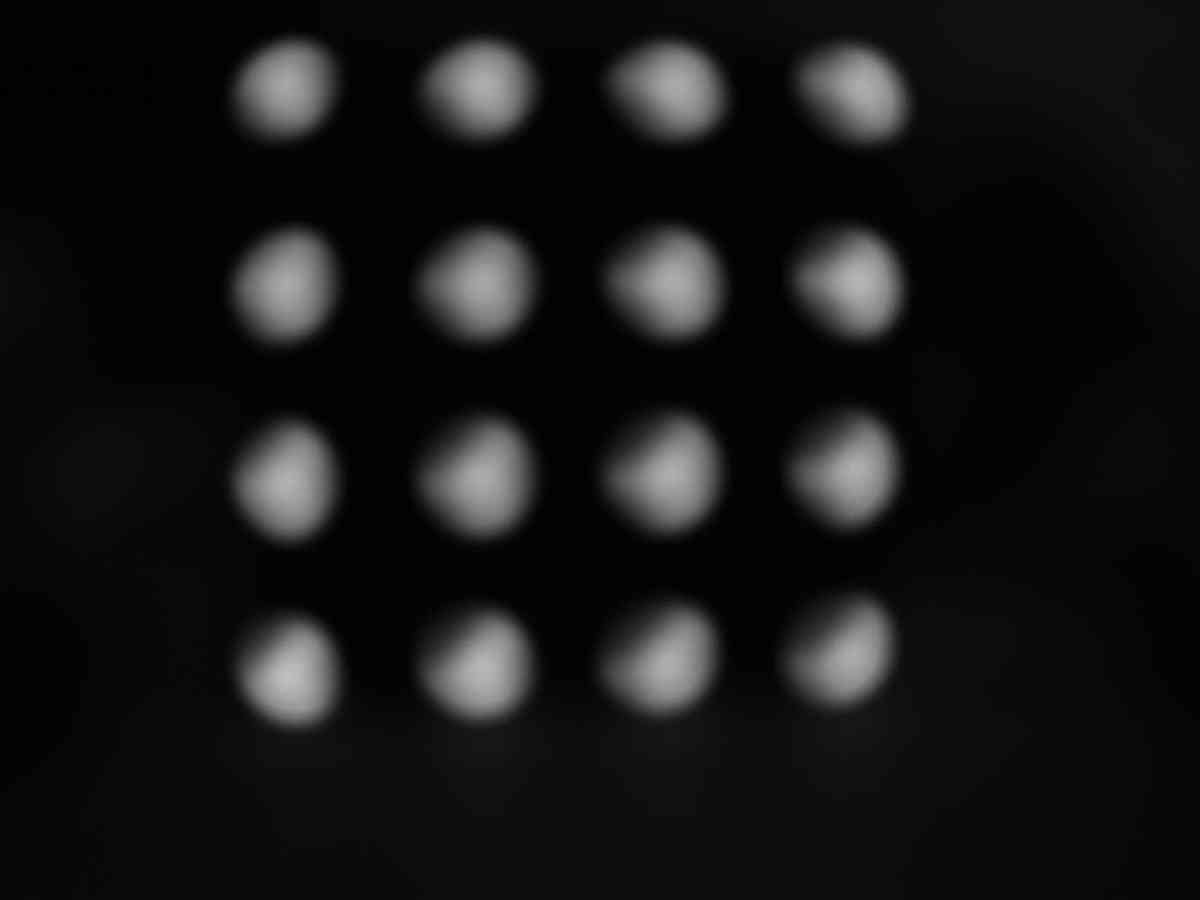
\includegraphics[height=20em]{../images/blurry.jpg}
    \vspace{-1.0em}
    \captionof{figure}{Verschwommene LEDs}
    \label{img:Verschwommene-LEDs}
\end{centering}

\begin{longtable}[c]{ @{} >{\RaggedRight\hspace{0pt}} lrrrrrl @{} }
    Kamera & $f_K$ [Hz] & $f_G$ [Hz] & $\bar f$ [Hz] & $b_K$ [µs] & $\bar t$ [µs] & Bilder in \appref{app:results}  % & FPS & Belichtungszeit
    \\\hline
      \hyperlinkXY{hyp:IDS} (verschwommen) & 59.99 & 59.701 & 59.974 & 4999 & 5018 & \hyperlinkXY{hyp:k-ueye-59-7-blur}
    \\\hyperlinkXY{hyp:A52} (Rolling Shutter) & 60.00 & 59.701 & 59.792 & ca. 10000 & 9921 & \hyperlinkXY{hyp:b-a52-59-7-rolling}
\end{longtable}
\captionof{table}{Auswertung bei schlechter Bildqualität}
\label{table:Auswertung-Bildqualität}

\subsubsection{Einfluss der Kalibration}

Aus den Bildern in \appref{app:results} erschliesst sich, dass die Kalibration die Messungen zum grössten Teil ein wenig verschäft.
Die FPS verschiebt sich im besten Fall sehr wenig (\imgref{img:fps-ot}), die Belichtungszeit wird schmaler (\imgref{img:exposure-ot}) und die Belichtungszeit zu Winkel werden ausgeglichener (\imgref{img:vs}).
Als Beispiel sind die Bilder aus \appref{app:results} \hyperlinkXY{hyp:k-ueye-60-3} gezeigt.
Die blauen Daten sind korrigiert und die orangenen sind die Rohdaten welche die Kalibration ignorieren.

\noindent\begin{minipage}[t]{\dimexpr.994\linewidth/3}\vspace{0pt}
    \begin{centering}
        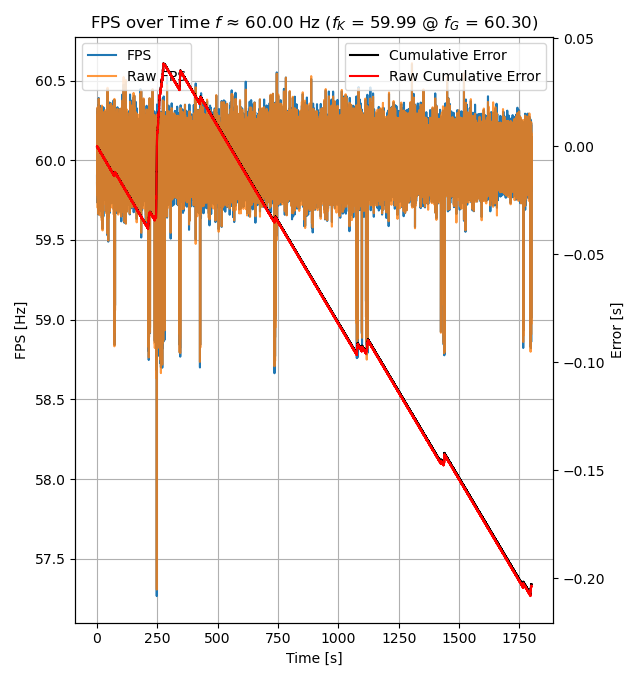
\includegraphics[width=\linewidth]{../results/59-99fps-4999us-at-60-299084fps-fps-both}
        \vspace{-2.0em}
        \captionof{figure}{FPS über Zeit}
        \label{img:fps-ot}
    \end{centering}
\end{minipage}
\noindent\begin{minipage}[t]{\dimexpr.994\linewidth/3}\vspace{0pt}
    \begin{centering}
        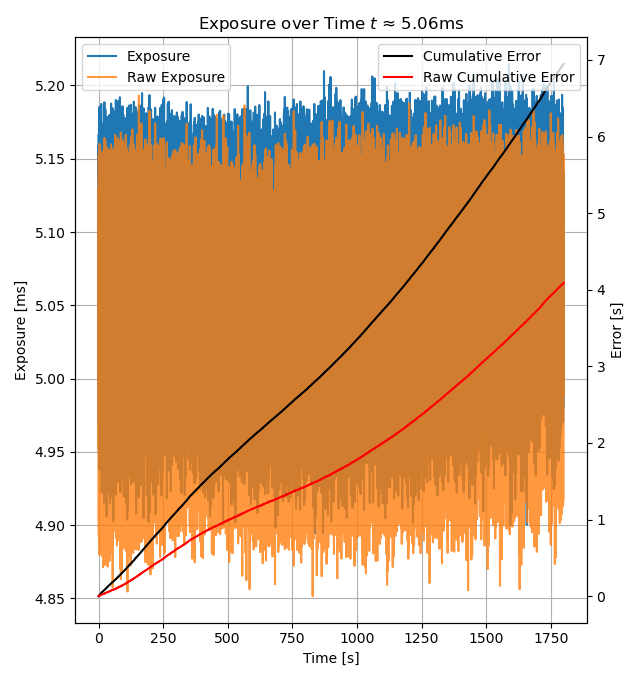
\includegraphics[width=\linewidth]{../results/59-99fps-4999us-at-60-299084fps-exposure-both}
        \vspace{-2.0em}
        \captionof{figure}{Belichtung über Zeit}
        \label{img:exposure-ot}
    \end{centering}
\end{minipage}
\noindent\begin{minipage}[t]{\dimexpr.994\linewidth/3}\vspace{0pt}
    \begin{centering}
        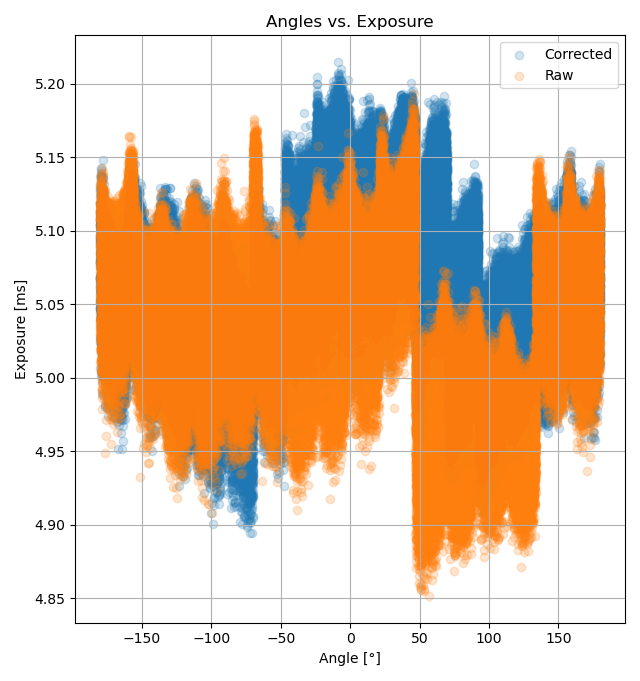
\includegraphics[width=\linewidth]{../results/59-99fps-4999us-at-60-299084fps-vs-both}
        \vspace{-2.0em}
        \captionof{figure}{Belichtung zu Winkel}
        \label{img:vs}
    \end{centering}
\end{minipage}


